% Options for packages loaded elsewhere
\PassOptionsToPackage{unicode}{hyperref}
\PassOptionsToPackage{hyphens}{url}
\PassOptionsToPackage{dvipsnames,svgnames,x11names}{xcolor}
%
\documentclass[
  letterpaper,
  DIV=11,
  numbers=noendperiod]{scrartcl}

\usepackage{amsmath,amssymb}
\usepackage{iftex}
\ifPDFTeX
  \usepackage[T1]{fontenc}
  \usepackage[utf8]{inputenc}
  \usepackage{textcomp} % provide euro and other symbols
\else % if luatex or xetex
  \usepackage{unicode-math}
  \defaultfontfeatures{Scale=MatchLowercase}
  \defaultfontfeatures[\rmfamily]{Ligatures=TeX,Scale=1}
\fi
\usepackage{lmodern}
\ifPDFTeX\else  
    % xetex/luatex font selection
\fi
% Use upquote if available, for straight quotes in verbatim environments
\IfFileExists{upquote.sty}{\usepackage{upquote}}{}
\IfFileExists{microtype.sty}{% use microtype if available
  \usepackage[]{microtype}
  \UseMicrotypeSet[protrusion]{basicmath} % disable protrusion for tt fonts
}{}
\makeatletter
\@ifundefined{KOMAClassName}{% if non-KOMA class
  \IfFileExists{parskip.sty}{%
    \usepackage{parskip}
  }{% else
    \setlength{\parindent}{0pt}
    \setlength{\parskip}{6pt plus 2pt minus 1pt}}
}{% if KOMA class
  \KOMAoptions{parskip=half}}
\makeatother
\usepackage{xcolor}
\setlength{\emergencystretch}{3em} % prevent overfull lines
\setcounter{secnumdepth}{5}
% Make \paragraph and \subparagraph free-standing
\makeatletter
\ifx\paragraph\undefined\else
  \let\oldparagraph\paragraph
  \renewcommand{\paragraph}{
    \@ifstar
      \xxxParagraphStar
      \xxxParagraphNoStar
  }
  \newcommand{\xxxParagraphStar}[1]{\oldparagraph*{#1}\mbox{}}
  \newcommand{\xxxParagraphNoStar}[1]{\oldparagraph{#1}\mbox{}}
\fi
\ifx\subparagraph\undefined\else
  \let\oldsubparagraph\subparagraph
  \renewcommand{\subparagraph}{
    \@ifstar
      \xxxSubParagraphStar
      \xxxSubParagraphNoStar
  }
  \newcommand{\xxxSubParagraphStar}[1]{\oldsubparagraph*{#1}\mbox{}}
  \newcommand{\xxxSubParagraphNoStar}[1]{\oldsubparagraph{#1}\mbox{}}
\fi
\makeatother

\usepackage{color}
\usepackage{fancyvrb}
\newcommand{\VerbBar}{|}
\newcommand{\VERB}{\Verb[commandchars=\\\{\}]}
\DefineVerbatimEnvironment{Highlighting}{Verbatim}{commandchars=\\\{\}}
% Add ',fontsize=\small' for more characters per line
\usepackage{framed}
\definecolor{shadecolor}{RGB}{241,243,245}
\newenvironment{Shaded}{\begin{snugshade}}{\end{snugshade}}
\newcommand{\AlertTok}[1]{\textcolor[rgb]{0.68,0.00,0.00}{#1}}
\newcommand{\AnnotationTok}[1]{\textcolor[rgb]{0.37,0.37,0.37}{#1}}
\newcommand{\AttributeTok}[1]{\textcolor[rgb]{0.40,0.45,0.13}{#1}}
\newcommand{\BaseNTok}[1]{\textcolor[rgb]{0.68,0.00,0.00}{#1}}
\newcommand{\BuiltInTok}[1]{\textcolor[rgb]{0.00,0.23,0.31}{#1}}
\newcommand{\CharTok}[1]{\textcolor[rgb]{0.13,0.47,0.30}{#1}}
\newcommand{\CommentTok}[1]{\textcolor[rgb]{0.37,0.37,0.37}{#1}}
\newcommand{\CommentVarTok}[1]{\textcolor[rgb]{0.37,0.37,0.37}{\textit{#1}}}
\newcommand{\ConstantTok}[1]{\textcolor[rgb]{0.56,0.35,0.01}{#1}}
\newcommand{\ControlFlowTok}[1]{\textcolor[rgb]{0.00,0.23,0.31}{\textbf{#1}}}
\newcommand{\DataTypeTok}[1]{\textcolor[rgb]{0.68,0.00,0.00}{#1}}
\newcommand{\DecValTok}[1]{\textcolor[rgb]{0.68,0.00,0.00}{#1}}
\newcommand{\DocumentationTok}[1]{\textcolor[rgb]{0.37,0.37,0.37}{\textit{#1}}}
\newcommand{\ErrorTok}[1]{\textcolor[rgb]{0.68,0.00,0.00}{#1}}
\newcommand{\ExtensionTok}[1]{\textcolor[rgb]{0.00,0.23,0.31}{#1}}
\newcommand{\FloatTok}[1]{\textcolor[rgb]{0.68,0.00,0.00}{#1}}
\newcommand{\FunctionTok}[1]{\textcolor[rgb]{0.28,0.35,0.67}{#1}}
\newcommand{\ImportTok}[1]{\textcolor[rgb]{0.00,0.46,0.62}{#1}}
\newcommand{\InformationTok}[1]{\textcolor[rgb]{0.37,0.37,0.37}{#1}}
\newcommand{\KeywordTok}[1]{\textcolor[rgb]{0.00,0.23,0.31}{\textbf{#1}}}
\newcommand{\NormalTok}[1]{\textcolor[rgb]{0.00,0.23,0.31}{#1}}
\newcommand{\OperatorTok}[1]{\textcolor[rgb]{0.37,0.37,0.37}{#1}}
\newcommand{\OtherTok}[1]{\textcolor[rgb]{0.00,0.23,0.31}{#1}}
\newcommand{\PreprocessorTok}[1]{\textcolor[rgb]{0.68,0.00,0.00}{#1}}
\newcommand{\RegionMarkerTok}[1]{\textcolor[rgb]{0.00,0.23,0.31}{#1}}
\newcommand{\SpecialCharTok}[1]{\textcolor[rgb]{0.37,0.37,0.37}{#1}}
\newcommand{\SpecialStringTok}[1]{\textcolor[rgb]{0.13,0.47,0.30}{#1}}
\newcommand{\StringTok}[1]{\textcolor[rgb]{0.13,0.47,0.30}{#1}}
\newcommand{\VariableTok}[1]{\textcolor[rgb]{0.07,0.07,0.07}{#1}}
\newcommand{\VerbatimStringTok}[1]{\textcolor[rgb]{0.13,0.47,0.30}{#1}}
\newcommand{\WarningTok}[1]{\textcolor[rgb]{0.37,0.37,0.37}{\textit{#1}}}

\providecommand{\tightlist}{%
  \setlength{\itemsep}{0pt}\setlength{\parskip}{0pt}}\usepackage{longtable,booktabs,array}
\usepackage{calc} % for calculating minipage widths
% Correct order of tables after \paragraph or \subparagraph
\usepackage{etoolbox}
\makeatletter
\patchcmd\longtable{\par}{\if@noskipsec\mbox{}\fi\par}{}{}
\makeatother
% Allow footnotes in longtable head/foot
\IfFileExists{footnotehyper.sty}{\usepackage{footnotehyper}}{\usepackage{footnote}}
\makesavenoteenv{longtable}
\usepackage{graphicx}
\makeatletter
\def\maxwidth{\ifdim\Gin@nat@width>\linewidth\linewidth\else\Gin@nat@width\fi}
\def\maxheight{\ifdim\Gin@nat@height>\textheight\textheight\else\Gin@nat@height\fi}
\makeatother
% Scale images if necessary, so that they will not overflow the page
% margins by default, and it is still possible to overwrite the defaults
% using explicit options in \includegraphics[width, height, ...]{}
\setkeys{Gin}{width=\maxwidth,height=\maxheight,keepaspectratio}
% Set default figure placement to htbp
\makeatletter
\def\fps@figure{htbp}
\makeatother

\KOMAoption{captions}{tableheading}
\makeatletter
\@ifpackageloaded{tcolorbox}{}{\usepackage[skins,breakable]{tcolorbox}}
\@ifpackageloaded{fontawesome5}{}{\usepackage{fontawesome5}}
\definecolor{quarto-callout-color}{HTML}{909090}
\definecolor{quarto-callout-note-color}{HTML}{0758E5}
\definecolor{quarto-callout-important-color}{HTML}{CC1914}
\definecolor{quarto-callout-warning-color}{HTML}{EB9113}
\definecolor{quarto-callout-tip-color}{HTML}{00A047}
\definecolor{quarto-callout-caution-color}{HTML}{FC5300}
\definecolor{quarto-callout-color-frame}{HTML}{acacac}
\definecolor{quarto-callout-note-color-frame}{HTML}{4582ec}
\definecolor{quarto-callout-important-color-frame}{HTML}{d9534f}
\definecolor{quarto-callout-warning-color-frame}{HTML}{f0ad4e}
\definecolor{quarto-callout-tip-color-frame}{HTML}{02b875}
\definecolor{quarto-callout-caution-color-frame}{HTML}{fd7e14}
\makeatother
\makeatletter
\@ifpackageloaded{caption}{}{\usepackage{caption}}
\AtBeginDocument{%
\ifdefined\contentsname
  \renewcommand*\contentsname{Table of contents}
\else
  \newcommand\contentsname{Table of contents}
\fi
\ifdefined\listfigurename
  \renewcommand*\listfigurename{List of Figures}
\else
  \newcommand\listfigurename{List of Figures}
\fi
\ifdefined\listtablename
  \renewcommand*\listtablename{List of Tables}
\else
  \newcommand\listtablename{List of Tables}
\fi
\ifdefined\figurename
  \renewcommand*\figurename{Figure}
\else
  \newcommand\figurename{Figure}
\fi
\ifdefined\tablename
  \renewcommand*\tablename{Table}
\else
  \newcommand\tablename{Table}
\fi
}
\@ifpackageloaded{float}{}{\usepackage{float}}
\floatstyle{ruled}
\@ifundefined{c@chapter}{\newfloat{codelisting}{h}{lop}}{\newfloat{codelisting}{h}{lop}[chapter]}
\floatname{codelisting}{Listing}
\newcommand*\listoflistings{\listof{codelisting}{List of Listings}}
\makeatother
\makeatletter
\makeatother
\makeatletter
\@ifpackageloaded{caption}{}{\usepackage{caption}}
\@ifpackageloaded{subcaption}{}{\usepackage{subcaption}}
\makeatother

\ifLuaTeX
  \usepackage{selnolig}  % disable illegal ligatures
\fi
\usepackage{bookmark}

\IfFileExists{xurl.sty}{\usepackage{xurl}}{} % add URL line breaks if available
\urlstyle{same} % disable monospaced font for URLs
\hypersetup{
  pdftitle={Palmer Penguins Data Analysis Series (Part 5): Random Forest vs Linear Models - The Final Comparison},
  pdfauthor={Your Name},
  colorlinks=true,
  linkcolor={blue},
  filecolor={Maroon},
  citecolor={Blue},
  urlcolor={Blue},
  pdfcreator={LaTeX via pandoc}}


\title{Palmer Penguins Data Analysis Series (Part 5): Random Forest vs
Linear Models - The Final Comparison}
\usepackage{etoolbox}
\makeatletter
\providecommand{\subtitle}[1]{% add subtitle to \maketitle
  \apptocmd{\@title}{\par {\large #1 \par}}{}{}
}
\makeatother
\subtitle{Settling the interpretability vs performance debate in
ecological modeling}
\author{Your Name}
\date{2025-01-05}

\begin{document}
\maketitle

\renewcommand*\contentsname{Table of contents}
{
\hypersetup{linkcolor=}
\setcounter{tocdepth}{3}
\tableofcontents
}

\begin{figure}[H]

{\centering 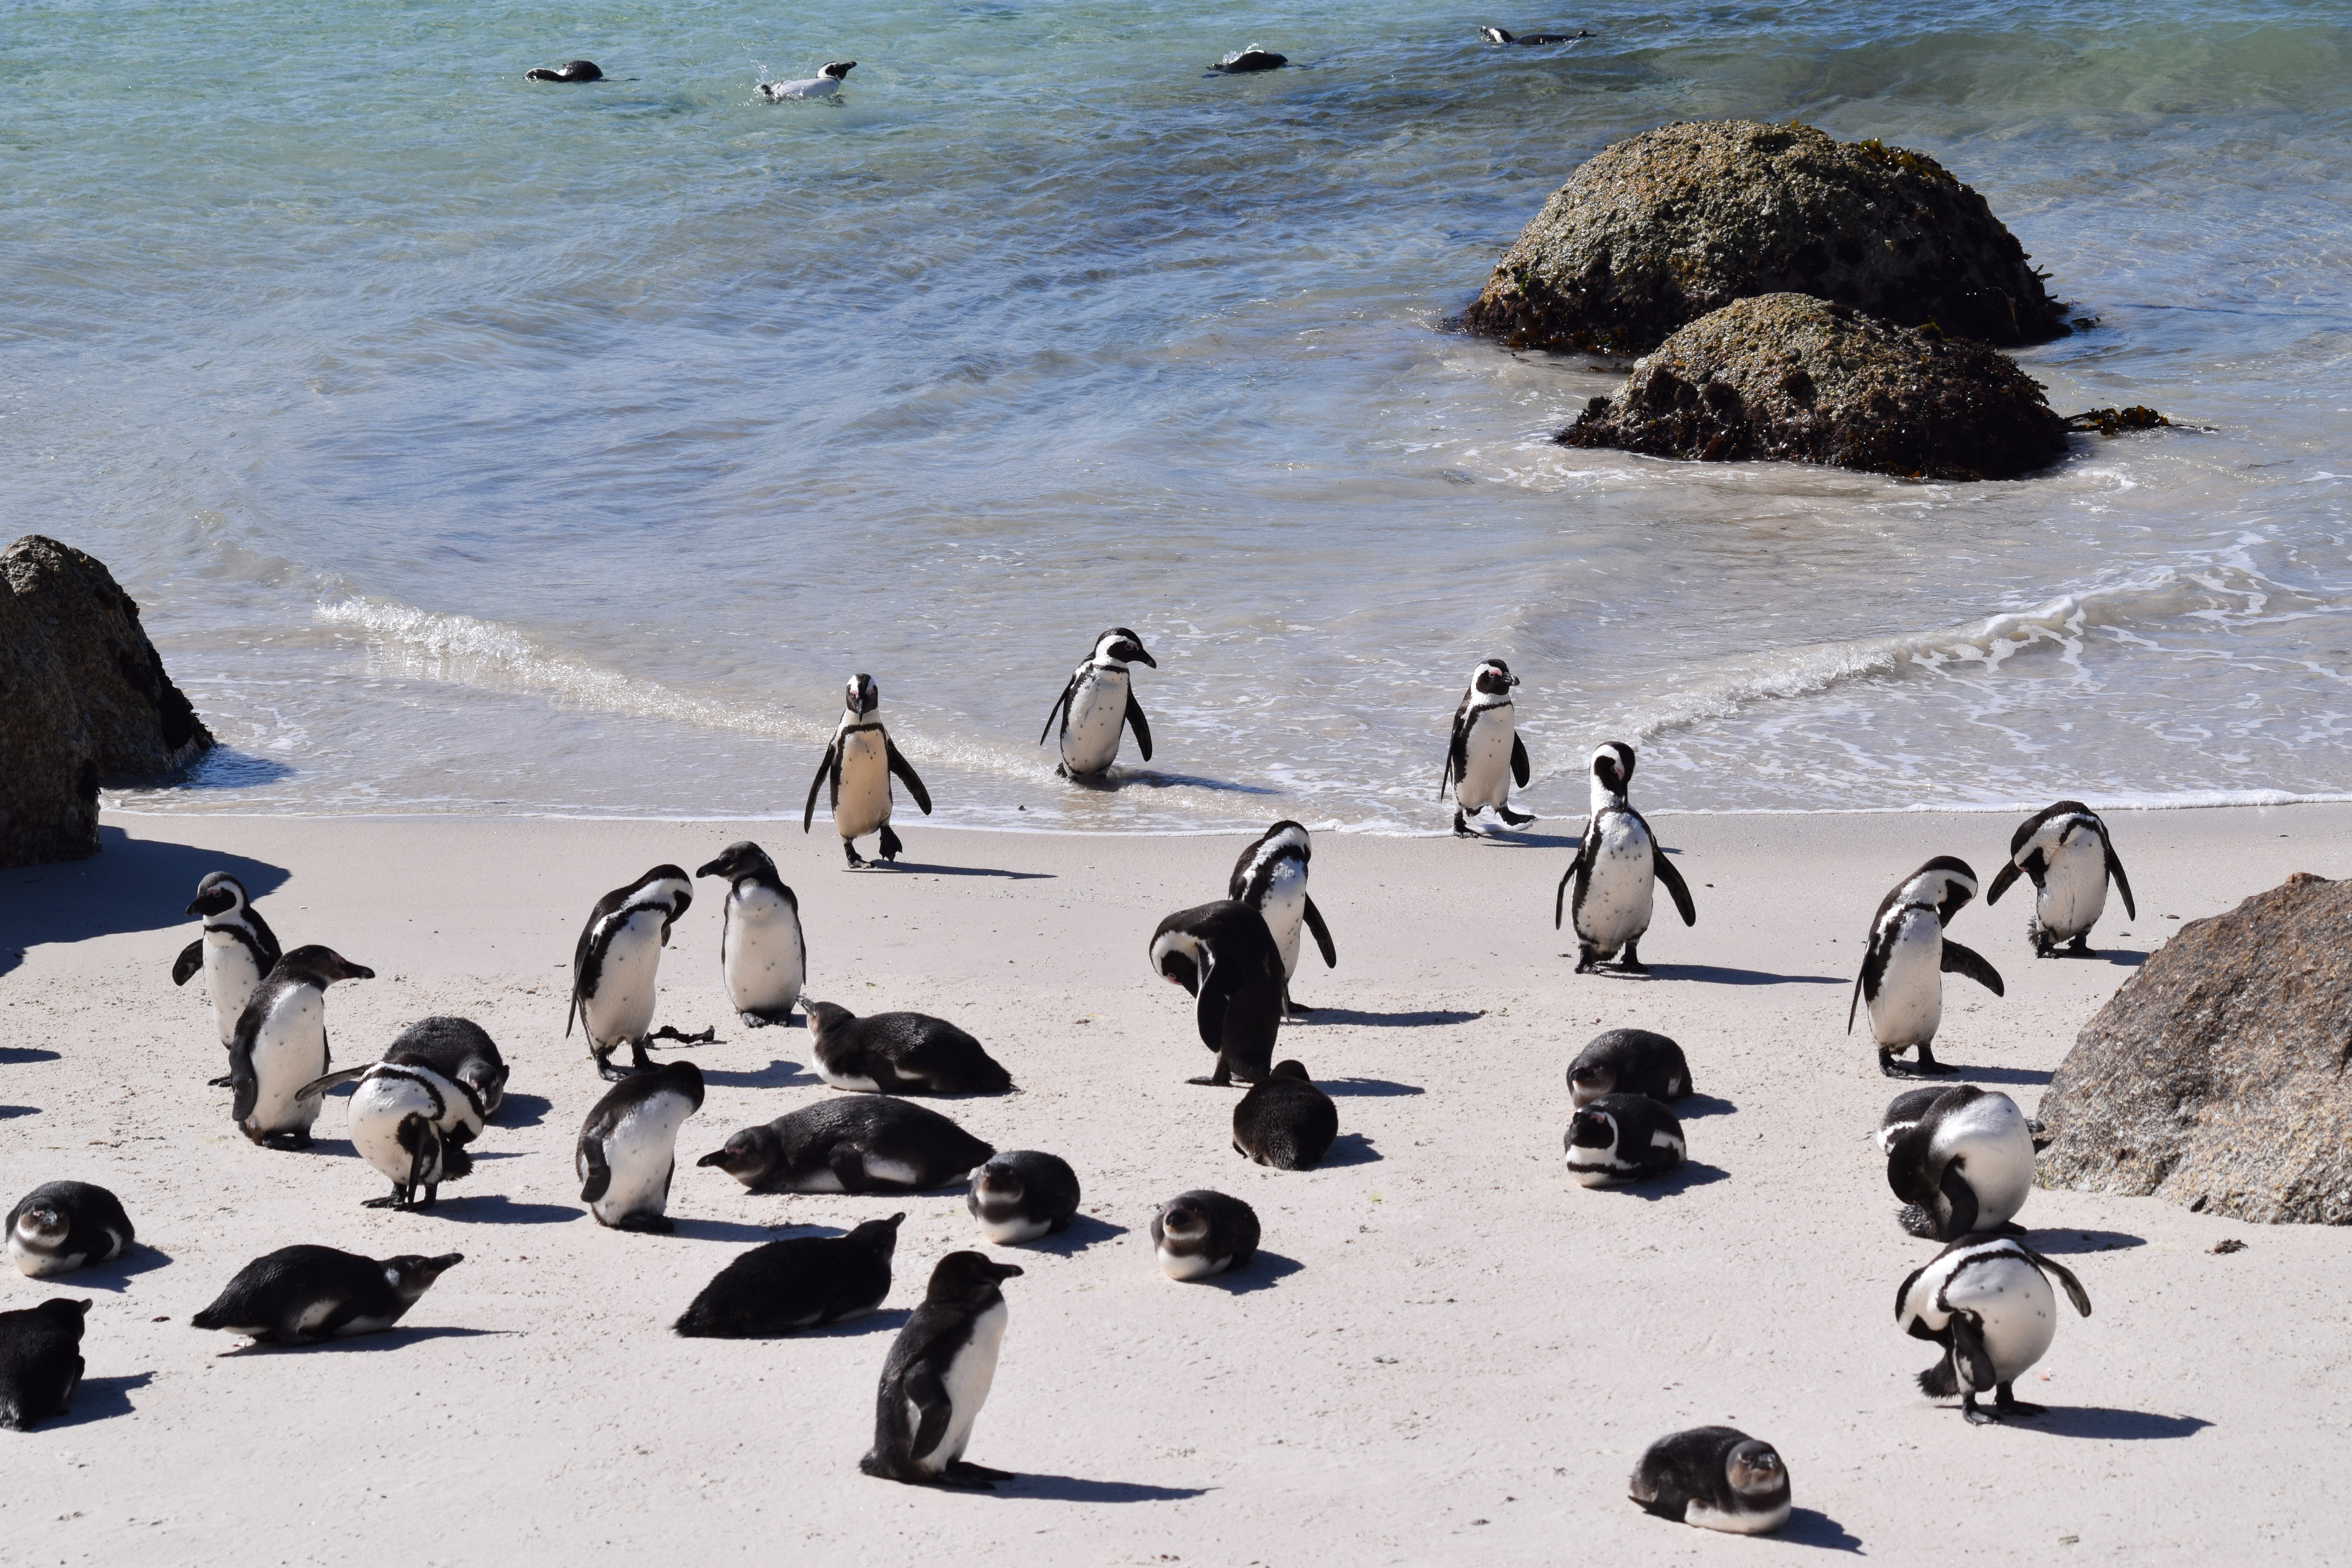
\includegraphics{../../images/posts/penguin-hero.jpg}

}

\caption{Two penguins at a crossroads - one holding a linear regression
equation, the other holding a decision tree, representing the classic
interpretability vs performance tradeoff!}

\end{figure}%

\emph{Photo: African penguins at Boulders Beach, South Africa. Licensed
under \href{https://creativecommons.org/licenses/by/2.0/}{CC BY 2.0} via
\href{https://commons.wikimedia.org/wiki/File:Boulders_Beach_penguins_(46475505885).jpg}{Wikimedia
Commons}}

\begin{tcolorbox}[enhanced jigsaw, bottomrule=.15mm, breakable, colback=white, arc=.35mm, colframe=quarto-callout-note-color-frame, left=2mm, rightrule=.15mm, toprule=.15mm, leftrule=.75mm, opacityback=0]
\begin{minipage}[t]{5.5mm}
\textcolor{quarto-callout-note-color}{\faInfo}
\end{minipage}%
\begin{minipage}[t]{\textwidth - 5.5mm}

\vspace{-3mm}\textbf{🐧 Palmer Penguins Data Analysis Series - FINALE}\vspace{3mm}

This is \textbf{Part 5} (Final) of our 5-part series exploring penguin
morphometrics:

\begin{enumerate}
\def\labelenumi{\arabic{enumi}.}
\tightlist
\item
  \href{../palmer_penguins_part1/}{Part 1: EDA and Simple Regression}
\item
  \href{../palmer_penguins_part2/}{Part 2: Multiple Regression and
  Species Effects}
\item
  \href{../palmer_penguins_part3/}{Part 3: Advanced Models and
  Cross-Validation}
\item
  \href{../palmer_penguins_part4/}{Part 4: Model Diagnostics and
  Interpretation}
\item
  \textbf{Part 5: Random Forest vs Linear Models} (This post - FINALE!)
\end{enumerate}

\end{minipage}%
\end{tcolorbox}

\section{Introduction}\label{introduction}

Welcome to the grand finale of our Palmer penguins data analysis
journey! We've traveled far together - from basic exploratory analysis
to sophisticated diagnostics, building and validating models that
explain 86\% of the variance in penguin body mass. But one crucial
question has been lurking beneath the surface throughout our journey:

\textbf{Should we sacrifice the beautiful interpretability of linear
models for potentially better predictive performance from machine
learning algorithms?}

This question sits at the heart of modern data science, especially in
scientific research where understanding \emph{why} is often as important
as predicting \emph{what}. Today, we'll conduct a comprehensive
head-to-head comparison between our carefully crafted linear models and
their machine learning challenger: random forests.

In this final post, we'll explore:

\begin{itemize}
\tightlist
\item
  Comprehensive performance comparison using multiple metrics
\item
  Feature importance analysis and partial dependence plots
\item
  The interpretability-performance tradeoff in action
\item
  Practical guidance for model selection in ecological research
\item
  When to choose linear models vs.~random forests
\item
  Best practices for communicating model choices to stakeholders
\end{itemize}

By the end of this series finale, you'll have a complete framework for
making informed decisions about model complexity in your own research.

\section{Setup and Model Arsenal}\label{setup-and-model-arsenal}

Let's assemble our complete modeling toolkit and establish fair
comparison conditions:

\begin{Shaded}
\begin{Highlighting}[]
\FunctionTok{library}\NormalTok{(palmerpenguins)}
\FunctionTok{library}\NormalTok{(tidyverse)}
\FunctionTok{library}\NormalTok{(randomForest)}
\FunctionTok{library}\NormalTok{(caret)}
\FunctionTok{library}\NormalTok{(broom)}
\FunctionTok{library}\NormalTok{(knitr)}
\FunctionTok{library}\NormalTok{(patchwork)}

\CommentTok{\# Conditional loading of optional packages}
\NormalTok{optional\_packages }\OtherTok{\textless{}{-}} \FunctionTok{c}\NormalTok{(}\StringTok{"pdp"}\NormalTok{, }\StringTok{"vip"}\NormalTok{, }\StringTok{"DALEX"}\NormalTok{)}
\ControlFlowTok{for}\NormalTok{ (pkg }\ControlFlowTok{in}\NormalTok{ optional\_packages) \{}
  \ControlFlowTok{if}\NormalTok{ (}\FunctionTok{requireNamespace}\NormalTok{(pkg, }\AttributeTok{quietly =} \ConstantTok{TRUE}\NormalTok{)) \{}
    \FunctionTok{library}\NormalTok{(pkg, }\AttributeTok{character.only =} \ConstantTok{TRUE}\NormalTok{)}
    \FunctionTok{cat}\NormalTok{(}\StringTok{"[OK] Loaded"}\NormalTok{, pkg, }\StringTok{"}\SpecialCharTok{\textbackslash{}n}\StringTok{"}\NormalTok{)}
\NormalTok{  \} }\ControlFlowTok{else}\NormalTok{ \{}
    \FunctionTok{cat}\NormalTok{(}\StringTok{"[INFO] Package \textquotesingle{}"}\NormalTok{, pkg, }\StringTok{"\textquotesingle{} not available. Install with: install.packages(\textquotesingle{}"}\NormalTok{, pkg, }\StringTok{"\textquotesingle{})}\SpecialCharTok{\textbackslash{}n}\StringTok{"}\NormalTok{)}
\NormalTok{  \}}
\NormalTok{\}}
\end{Highlighting}
\end{Shaded}

\begin{verbatim}
[INFO] Package ' pdp ' not available. Install with: install.packages(' pdp ')
[INFO] Package ' vip ' not available. Install with: install.packages(' vip ')
[INFO] Package ' DALEX ' not available. Install with: install.packages(' DALEX ')
\end{verbatim}

\begin{Shaded}
\begin{Highlighting}[]
\CommentTok{\# Set theme and colors}
\FunctionTok{theme\_set}\NormalTok{(}\FunctionTok{theme\_minimal}\NormalTok{(}\AttributeTok{base\_size =} \DecValTok{12}\NormalTok{))}
\NormalTok{penguin\_colors }\OtherTok{\textless{}{-}} \FunctionTok{c}\NormalTok{(}\StringTok{"Adelie"} \OtherTok{=} \StringTok{"\#FF6B6B"}\NormalTok{, }\StringTok{"Chinstrap"} \OtherTok{=} \StringTok{"\#4ECDC4"}\NormalTok{, }\StringTok{"Gentoo"} \OtherTok{=} \StringTok{"\#45B7D1"}\NormalTok{)}

\CommentTok{\# Load and prepare data}
\FunctionTok{data}\NormalTok{(penguins)}
\NormalTok{penguins\_clean }\OtherTok{\textless{}{-}}\NormalTok{ penguins }\SpecialCharTok{\%\textgreater{}\%} \FunctionTok{drop\_na}\NormalTok{()}

\CommentTok{\# Set seed for reproducibility}
\FunctionTok{set.seed}\NormalTok{(}\DecValTok{42}\NormalTok{)}

\FunctionTok{cat}\NormalTok{(}\StringTok{"=== FINALE: The Ultimate Model Comparison ===}\SpecialCharTok{\textbackslash{}n}\StringTok{"}\NormalTok{)}
\end{Highlighting}
\end{Shaded}

\begin{verbatim}
=== FINALE: The Ultimate Model Comparison ===
\end{verbatim}

\begin{Shaded}
\begin{Highlighting}[]
\FunctionTok{cat}\NormalTok{(}\StringTok{"============================================}\SpecialCharTok{\textbackslash{}n}\StringTok{"}\NormalTok{)}
\end{Highlighting}
\end{Shaded}

\begin{verbatim}
============================================
\end{verbatim}

\begin{Shaded}
\begin{Highlighting}[]
\FunctionTok{cat}\NormalTok{(}\FunctionTok{sprintf}\NormalTok{(}\StringTok{"Dataset: \%d penguins across \%d variables}\SpecialCharTok{\textbackslash{}n}\StringTok{"}\NormalTok{, }\FunctionTok{nrow}\NormalTok{(penguins\_clean), }\FunctionTok{ncol}\NormalTok{(penguins\_clean)))}
\end{Highlighting}
\end{Shaded}

\begin{verbatim}
Dataset: 333 penguins across 8 variables
\end{verbatim}

\begin{Shaded}
\begin{Highlighting}[]
\FunctionTok{cat}\NormalTok{(}\StringTok{"Comparison: Linear Models vs Random Forests}\SpecialCharTok{\textbackslash{}n}\StringTok{"}\NormalTok{)}
\end{Highlighting}
\end{Shaded}

\begin{verbatim}
Comparison: Linear Models vs Random Forests
\end{verbatim}

\begin{Shaded}
\begin{Highlighting}[]
\FunctionTok{cat}\NormalTok{(}\StringTok{"Evaluation: Cross{-}validation with multiple metrics}\SpecialCharTok{\textbackslash{}n}\StringTok{"}\NormalTok{)}
\end{Highlighting}
\end{Shaded}

\begin{verbatim}
Evaluation: Cross-validation with multiple metrics
\end{verbatim}

\begin{Shaded}
\begin{Highlighting}[]
\FunctionTok{cat}\NormalTok{(}\StringTok{"Goal: Determine optimal approach for ecological modeling}\SpecialCharTok{\textbackslash{}n}\StringTok{"}\NormalTok{)}
\end{Highlighting}
\end{Shaded}

\begin{verbatim}
Goal: Determine optimal approach for ecological modeling
\end{verbatim}

\section{Comprehensive Model
Training}\label{comprehensive-model-training}

Let's train our complete arsenal of models using identical
cross-validation procedures:

\subsection{Cross-Validation Setup}\label{cross-validation-setup}

\begin{Shaded}
\begin{Highlighting}[]
\CommentTok{\# Consistent cross{-}validation setup}
\NormalTok{train\_control }\OtherTok{\textless{}{-}} \FunctionTok{trainControl}\NormalTok{(}
  \AttributeTok{method =} \StringTok{"cv"}\NormalTok{,}
  \AttributeTok{number =} \DecValTok{10}\NormalTok{,}
  \AttributeTok{savePredictions =} \StringTok{"final"}\NormalTok{,}
  \AttributeTok{verboseIter =} \ConstantTok{FALSE}
\NormalTok{)}

\FunctionTok{cat}\NormalTok{(}\StringTok{"{-}{-}{-} Experimental Design {-}{-}{-}}\SpecialCharTok{\textbackslash{}n}\StringTok{"}\NormalTok{)}
\end{Highlighting}
\end{Shaded}

\begin{verbatim}
--- Experimental Design ---
\end{verbatim}

\begin{Shaded}
\begin{Highlighting}[]
\FunctionTok{cat}\NormalTok{(}\StringTok{"=======================}\SpecialCharTok{\textbackslash{}n}\StringTok{"}\NormalTok{)}
\end{Highlighting}
\end{Shaded}

\begin{verbatim}
=======================
\end{verbatim}

\begin{Shaded}
\begin{Highlighting}[]
\FunctionTok{cat}\NormalTok{(}\StringTok{"Cross{-}validation: 10{-}fold}\SpecialCharTok{\textbackslash{}n}\StringTok{"}\NormalTok{)}
\end{Highlighting}
\end{Shaded}

\begin{verbatim}
Cross-validation: 10-fold
\end{verbatim}

\begin{Shaded}
\begin{Highlighting}[]
\FunctionTok{cat}\NormalTok{(}\StringTok{"Seed: 42 (consistent across all models)}\SpecialCharTok{\textbackslash{}n}\StringTok{"}\NormalTok{)}
\end{Highlighting}
\end{Shaded}

\begin{verbatim}
Seed: 42 (consistent across all models)
\end{verbatim}

\begin{Shaded}
\begin{Highlighting}[]
\FunctionTok{cat}\NormalTok{(}\StringTok{"Metrics: RMSE, R{-}squared, MAE}\SpecialCharTok{\textbackslash{}n}\StringTok{"}\NormalTok{)}
\end{Highlighting}
\end{Shaded}

\begin{verbatim}
Metrics: RMSE, R-squared, MAE
\end{verbatim}

\begin{Shaded}
\begin{Highlighting}[]
\FunctionTok{cat}\NormalTok{(}\StringTok{"Evaluation: Performance + interpretability}\SpecialCharTok{\textbackslash{}n}\StringTok{"}\NormalTok{)}
\end{Highlighting}
\end{Shaded}

\begin{verbatim}
Evaluation: Performance + interpretability
\end{verbatim}

\subsection{Linear Model Variants}\label{linear-model-variants}

\begin{Shaded}
\begin{Highlighting}[]
\CommentTok{\# Simple linear model}
\NormalTok{linear\_simple }\OtherTok{\textless{}{-}} \FunctionTok{train}\NormalTok{(}
\NormalTok{  body\_mass\_g }\SpecialCharTok{\textasciitilde{}}\NormalTok{ flipper\_length\_mm,}
  \AttributeTok{data =}\NormalTok{ penguins\_clean,}
  \AttributeTok{method =} \StringTok{"lm"}\NormalTok{,}
  \AttributeTok{trControl =}\NormalTok{ train\_control}
\NormalTok{)}

\CommentTok{\# Multiple regression}
\NormalTok{linear\_multiple }\OtherTok{\textless{}{-}} \FunctionTok{train}\NormalTok{(}
\NormalTok{  body\_mass\_g }\SpecialCharTok{\textasciitilde{}}\NormalTok{ bill\_length\_mm }\SpecialCharTok{+}\NormalTok{ bill\_depth\_mm }\SpecialCharTok{+}\NormalTok{ flipper\_length\_mm,}
  \AttributeTok{data =}\NormalTok{ penguins\_clean,}
  \AttributeTok{method =} \StringTok{"lm"}\NormalTok{, }
  \AttributeTok{trControl =}\NormalTok{ train\_control}
\NormalTok{)}

\CommentTok{\# Species{-}aware model (our champion from previous parts)}
\NormalTok{linear\_species }\OtherTok{\textless{}{-}} \FunctionTok{train}\NormalTok{(}
\NormalTok{  body\_mass\_g }\SpecialCharTok{\textasciitilde{}}\NormalTok{ bill\_length\_mm }\SpecialCharTok{+}\NormalTok{ bill\_depth\_mm }\SpecialCharTok{+}\NormalTok{ flipper\_length\_mm }\SpecialCharTok{+}\NormalTok{ species,}
  \AttributeTok{data =}\NormalTok{ penguins\_clean,}
  \AttributeTok{method =} \StringTok{"lm"}\NormalTok{,}
  \AttributeTok{trControl =}\NormalTok{ train\_control}
\NormalTok{)}

\CommentTok{\# Polynomial model}
\NormalTok{linear\_poly }\OtherTok{\textless{}{-}} \FunctionTok{train}\NormalTok{(}
\NormalTok{  body\_mass\_g }\SpecialCharTok{\textasciitilde{}} \FunctionTok{poly}\NormalTok{(flipper\_length\_mm, }\DecValTok{2}\NormalTok{) }\SpecialCharTok{+} \FunctionTok{poly}\NormalTok{(bill\_length\_mm, }\DecValTok{2}\NormalTok{) }\SpecialCharTok{+} 
                \FunctionTok{poly}\NormalTok{(bill\_depth\_mm, }\DecValTok{2}\NormalTok{) }\SpecialCharTok{+}\NormalTok{ species,}
  \AttributeTok{data =}\NormalTok{ penguins\_clean,}
  \AttributeTok{method =} \StringTok{"lm"}\NormalTok{,}
  \AttributeTok{trControl =}\NormalTok{ train\_control}
\NormalTok{)}

\FunctionTok{cat}\NormalTok{(}\StringTok{"[OK] Linear models trained:}\SpecialCharTok{\textbackslash{}n}\StringTok{"}\NormalTok{)}
\end{Highlighting}
\end{Shaded}

\begin{verbatim}
[OK] Linear models trained:
\end{verbatim}

\begin{Shaded}
\begin{Highlighting}[]
\FunctionTok{cat}\NormalTok{(}\StringTok{"• Simple (flipper only)}\SpecialCharTok{\textbackslash{}n}\StringTok{"}\NormalTok{)}
\end{Highlighting}
\end{Shaded}

\begin{verbatim}
• Simple (flipper only)
\end{verbatim}

\begin{Shaded}
\begin{Highlighting}[]
\FunctionTok{cat}\NormalTok{(}\StringTok{"• Multiple (all morphometrics)}\SpecialCharTok{\textbackslash{}n}\StringTok{"}\NormalTok{) }
\end{Highlighting}
\end{Shaded}

\begin{verbatim}
• Multiple (all morphometrics)
\end{verbatim}

\begin{Shaded}
\begin{Highlighting}[]
\FunctionTok{cat}\NormalTok{(}\StringTok{"• Species{-}aware (morphometrics + species)}\SpecialCharTok{\textbackslash{}n}\StringTok{"}\NormalTok{)}
\end{Highlighting}
\end{Shaded}

\begin{verbatim}
• Species-aware (morphometrics + species)
\end{verbatim}

\begin{Shaded}
\begin{Highlighting}[]
\FunctionTok{cat}\NormalTok{(}\StringTok{"• Polynomial (quadratic features + species)}\SpecialCharTok{\textbackslash{}n}\StringTok{"}\NormalTok{)}
\end{Highlighting}
\end{Shaded}

\begin{verbatim}
• Polynomial (quadratic features + species)
\end{verbatim}

\subsection{Random Forest Variants}\label{random-forest-variants}

\begin{Shaded}
\begin{Highlighting}[]
\CommentTok{\# Basic random forest (morphometrics only)}
\NormalTok{rf\_basic }\OtherTok{\textless{}{-}} \FunctionTok{train}\NormalTok{(}
\NormalTok{  body\_mass\_g }\SpecialCharTok{\textasciitilde{}}\NormalTok{ bill\_length\_mm }\SpecialCharTok{+}\NormalTok{ bill\_depth\_mm }\SpecialCharTok{+}\NormalTok{ flipper\_length\_mm,}
  \AttributeTok{data =}\NormalTok{ penguins\_clean,}
  \AttributeTok{method =} \StringTok{"rf"}\NormalTok{,}
  \AttributeTok{trControl =}\NormalTok{ train\_control,}
  \AttributeTok{ntree =} \DecValTok{500}\NormalTok{,}
  \AttributeTok{importance =} \ConstantTok{TRUE}
\NormalTok{)}
\end{Highlighting}
\end{Shaded}

\begin{verbatim}
note: only 2 unique complexity parameters in default grid. Truncating the grid to 2 .
\end{verbatim}

\begin{Shaded}
\begin{Highlighting}[]
\CommentTok{\# Full random forest (all available predictors)}
\NormalTok{rf\_full }\OtherTok{\textless{}{-}} \FunctionTok{train}\NormalTok{(}
\NormalTok{  body\_mass\_g }\SpecialCharTok{\textasciitilde{}}\NormalTok{ bill\_length\_mm }\SpecialCharTok{+}\NormalTok{ bill\_depth\_mm }\SpecialCharTok{+}\NormalTok{ flipper\_length\_mm }\SpecialCharTok{+} 
\NormalTok{                species }\SpecialCharTok{+}\NormalTok{ sex }\SpecialCharTok{+}\NormalTok{ island }\SpecialCharTok{+}\NormalTok{ year,}
  \AttributeTok{data =}\NormalTok{ penguins\_clean,}
  \AttributeTok{method =} \StringTok{"rf"}\NormalTok{,}
  \AttributeTok{trControl =}\NormalTok{ train\_control,}
  \AttributeTok{ntree =} \DecValTok{500}\NormalTok{,}
  \AttributeTok{importance =} \ConstantTok{TRUE}
\NormalTok{)}

\CommentTok{\# Tuned random forest (optimized hyperparameters)}
\NormalTok{rf\_tuned }\OtherTok{\textless{}{-}} \FunctionTok{train}\NormalTok{(}
\NormalTok{  body\_mass\_g }\SpecialCharTok{\textasciitilde{}}\NormalTok{ bill\_length\_mm }\SpecialCharTok{+}\NormalTok{ bill\_depth\_mm }\SpecialCharTok{+}\NormalTok{ flipper\_length\_mm }\SpecialCharTok{+} 
\NormalTok{                species }\SpecialCharTok{+}\NormalTok{ sex }\SpecialCharTok{+}\NormalTok{ island,}
  \AttributeTok{data =}\NormalTok{ penguins\_clean,}
  \AttributeTok{method =} \StringTok{"rf"}\NormalTok{,}
  \AttributeTok{trControl =}\NormalTok{ train\_control,}
  \AttributeTok{tuneGrid =} \FunctionTok{expand.grid}\NormalTok{(}\AttributeTok{mtry =} \FunctionTok{c}\NormalTok{(}\DecValTok{2}\NormalTok{, }\DecValTok{3}\NormalTok{, }\DecValTok{4}\NormalTok{, }\DecValTok{5}\NormalTok{)),}
  \AttributeTok{ntree =} \DecValTok{500}\NormalTok{,}
  \AttributeTok{importance =} \ConstantTok{TRUE}
\NormalTok{)}

\FunctionTok{cat}\NormalTok{(}\StringTok{"}\SpecialCharTok{\textbackslash{}n}\StringTok{[OK] Random forest models trained:}\SpecialCharTok{\textbackslash{}n}\StringTok{"}\NormalTok{)}
\end{Highlighting}
\end{Shaded}

\begin{verbatim}

[OK] Random forest models trained:
\end{verbatim}

\begin{Shaded}
\begin{Highlighting}[]
\FunctionTok{cat}\NormalTok{(}\StringTok{"• Basic (morphometrics only)}\SpecialCharTok{\textbackslash{}n}\StringTok{"}\NormalTok{)}
\end{Highlighting}
\end{Shaded}

\begin{verbatim}
• Basic (morphometrics only)
\end{verbatim}

\begin{Shaded}
\begin{Highlighting}[]
\FunctionTok{cat}\NormalTok{(}\StringTok{"• Full (all predictors)}\SpecialCharTok{\textbackslash{}n}\StringTok{"}\NormalTok{)}
\end{Highlighting}
\end{Shaded}

\begin{verbatim}
• Full (all predictors)
\end{verbatim}

\begin{Shaded}
\begin{Highlighting}[]
\FunctionTok{cat}\NormalTok{(}\StringTok{"• Tuned (optimized hyperparameters)}\SpecialCharTok{\textbackslash{}n}\StringTok{"}\NormalTok{)}
\end{Highlighting}
\end{Shaded}

\begin{verbatim}
• Tuned (optimized hyperparameters)
\end{verbatim}

\section{Performance Comparison}\label{performance-comparison}

\subsection{Comprehensive Performance
Table}\label{comprehensive-performance-table}

\begin{Shaded}
\begin{Highlighting}[]
\CommentTok{\# Compile all models}
\NormalTok{all\_models }\OtherTok{\textless{}{-}} \FunctionTok{list}\NormalTok{(}
  \StringTok{"Linear: Simple"} \OtherTok{=}\NormalTok{ linear\_simple,}
  \StringTok{"Linear: Multiple"} \OtherTok{=}\NormalTok{ linear\_multiple,}
  \StringTok{"Linear: Species"} \OtherTok{=}\NormalTok{ linear\_species,}
  \StringTok{"Linear: Polynomial"} \OtherTok{=}\NormalTok{ linear\_poly,}
  \StringTok{"RF: Basic"} \OtherTok{=}\NormalTok{ rf\_basic,}
  \StringTok{"RF: Full"} \OtherTok{=}\NormalTok{ rf\_full,}
  \StringTok{"RF: Tuned"} \OtherTok{=}\NormalTok{ rf\_tuned}
\NormalTok{)}

\CommentTok{\# Extract performance metrics}
\NormalTok{performance\_comparison }\OtherTok{\textless{}{-}} \FunctionTok{map\_dfr}\NormalTok{(all\_models, }\ControlFlowTok{function}\NormalTok{(model) \{}
\NormalTok{  results }\OtherTok{\textless{}{-}}\NormalTok{ model}\SpecialCharTok{$}\NormalTok{results}
\NormalTok{  best\_idx }\OtherTok{\textless{}{-}} \FunctionTok{which.min}\NormalTok{(results}\SpecialCharTok{$}\NormalTok{RMSE)}
  
  \FunctionTok{data.frame}\NormalTok{(}
    \AttributeTok{RMSE\_mean =}\NormalTok{ results}\SpecialCharTok{$}\NormalTok{RMSE[best\_idx],}
    \AttributeTok{RMSE\_sd =} \FunctionTok{sd}\NormalTok{(model}\SpecialCharTok{$}\NormalTok{resample}\SpecialCharTok{$}\NormalTok{RMSE),}
    \AttributeTok{Rsquared\_mean =}\NormalTok{ results}\SpecialCharTok{$}\NormalTok{Rsquared[best\_idx],}
    \AttributeTok{Rsquared\_sd =} \FunctionTok{sd}\NormalTok{(model}\SpecialCharTok{$}\NormalTok{resample}\SpecialCharTok{$}\NormalTok{Rsquared),}
    \AttributeTok{MAE\_mean =}\NormalTok{ results}\SpecialCharTok{$}\NormalTok{MAE[best\_idx],}
    \AttributeTok{MAE\_sd =} \FunctionTok{sd}\NormalTok{(model}\SpecialCharTok{$}\NormalTok{resample}\SpecialCharTok{$}\NormalTok{MAE)}
\NormalTok{  )}
\NormalTok{\}, }\AttributeTok{.id =} \StringTok{"Model"}\NormalTok{) }\SpecialCharTok{\%\textgreater{}\%}
  \FunctionTok{arrange}\NormalTok{(RMSE\_mean) }\SpecialCharTok{\%\textgreater{}\%}
  \FunctionTok{mutate}\NormalTok{(}
    \AttributeTok{Rank =} \FunctionTok{row\_number}\NormalTok{(),}
    \AttributeTok{Model\_Type =} \FunctionTok{ifelse}\NormalTok{(}\FunctionTok{str\_detect}\NormalTok{(Model, }\StringTok{"Linear"}\NormalTok{), }\StringTok{"Linear"}\NormalTok{, }\StringTok{"Random Forest"}\NormalTok{)}
\NormalTok{  )}

\CommentTok{\# Format for display}
\NormalTok{performance\_display }\OtherTok{\textless{}{-}}\NormalTok{ performance\_comparison }\SpecialCharTok{\%\textgreater{}\%}
  \FunctionTok{mutate}\NormalTok{(}
    \AttributeTok{RMSE =} \FunctionTok{sprintf}\NormalTok{(}\StringTok{"\%.1f ± \%.1f"}\NormalTok{, RMSE\_mean, RMSE\_sd),}
    \AttributeTok{R\_squared =} \FunctionTok{sprintf}\NormalTok{(}\StringTok{"\%.3f ± \%.3f"}\NormalTok{, Rsquared\_mean, Rsquared\_sd),}
    \AttributeTok{MAE =} \FunctionTok{sprintf}\NormalTok{(}\StringTok{"\%.1f ± \%.1f"}\NormalTok{, MAE\_mean, MAE\_sd)}
\NormalTok{  ) }\SpecialCharTok{\%\textgreater{}\%}
  \FunctionTok{select}\NormalTok{(Rank, Model, Model\_Type, RMSE, R\_squared, MAE)}

\FunctionTok{kable}\NormalTok{(performance\_display,}
      \AttributeTok{caption =} \StringTok{"Complete Model Performance Comparison (Cross{-}Validated)"}\NormalTok{,}
      \AttributeTok{col.names =} \FunctionTok{c}\NormalTok{(}\StringTok{"Rank"}\NormalTok{, }\StringTok{"Model"}\NormalTok{, }\StringTok{"Type"}\NormalTok{, }\StringTok{"RMSE (g)"}\NormalTok{, }\StringTok{"R²"}\NormalTok{, }\StringTok{"MAE (g)"}\NormalTok{))}
\end{Highlighting}
\end{Shaded}

\begin{longtable}[]{@{}
  >{\raggedleft\arraybackslash}p{(\columnwidth - 10\tabcolsep) * \real{0.0641}}
  >{\raggedright\arraybackslash}p{(\columnwidth - 10\tabcolsep) * \real{0.2436}}
  >{\raggedright\arraybackslash}p{(\columnwidth - 10\tabcolsep) * \real{0.1795}}
  >{\raggedright\arraybackslash}p{(\columnwidth - 10\tabcolsep) * \real{0.1667}}
  >{\raggedright\arraybackslash}p{(\columnwidth - 10\tabcolsep) * \real{0.1795}}
  >{\raggedright\arraybackslash}p{(\columnwidth - 10\tabcolsep) * \real{0.1667}}@{}}
\caption{Complete Model Performance Comparison
(Cross-Validated)}\tabularnewline
\toprule\noalign{}
\begin{minipage}[b]{\linewidth}\raggedleft
Rank
\end{minipage} & \begin{minipage}[b]{\linewidth}\raggedright
Model
\end{minipage} & \begin{minipage}[b]{\linewidth}\raggedright
Type
\end{minipage} & \begin{minipage}[b]{\linewidth}\raggedright
RMSE (g)
\end{minipage} & \begin{minipage}[b]{\linewidth}\raggedright
R²
\end{minipage} & \begin{minipage}[b]{\linewidth}\raggedright
MAE (g)
\end{minipage} \\
\midrule\noalign{}
\endfirsthead
\toprule\noalign{}
\begin{minipage}[b]{\linewidth}\raggedleft
Rank
\end{minipage} & \begin{minipage}[b]{\linewidth}\raggedright
Model
\end{minipage} & \begin{minipage}[b]{\linewidth}\raggedright
Type
\end{minipage} & \begin{minipage}[b]{\linewidth}\raggedright
RMSE (g)
\end{minipage} & \begin{minipage}[b]{\linewidth}\raggedright
R²
\end{minipage} & \begin{minipage}[b]{\linewidth}\raggedright
MAE (g)
\end{minipage} \\
\midrule\noalign{}
\endhead
\bottomrule\noalign{}
\endlastfoot
1 & RF: Tuned & Random Forest & 294.9 ± 45.6 & 0.866 ± 0.050 & 235.9 ±
38.5 \\
2 & RF: Full & Random Forest & 296.0 ± 29.9 & 0.870 ± 0.024 & 236.7 ±
25.2 \\
3 & Linear: Polynomial & Linear & 310.3 ± 42.9 & 0.858 ± 0.035 & 249.4 ±
34.1 \\
4 & Linear: Species & Linear & 315.7 ± 32.2 & 0.856 ± 0.022 & 251.6 ±
24.8 \\
5 & RF: Basic & Random Forest & 341.4 ± 36.2 & 0.827 ± 0.042 & 269.0 ±
38.7 \\
6 & Linear: Simple & Linear & 390.9 ± 54.0 & 0.775 ± 0.038 & 314.1 ±
42.9 \\
7 & Linear: Multiple & Linear & 392.6 ± 41.7 & 0.769 ± 0.049 & 312.9 ±
27.3 \\
\end{longtable}

\begin{Shaded}
\begin{Highlighting}[]
\CommentTok{\# Identify top performers}
\NormalTok{top\_linear }\OtherTok{\textless{}{-}}\NormalTok{ performance\_comparison }\SpecialCharTok{\%\textgreater{}\%} \FunctionTok{filter}\NormalTok{(Model\_Type }\SpecialCharTok{==} \StringTok{"Linear"}\NormalTok{) }\SpecialCharTok{\%\textgreater{}\%} \FunctionTok{slice\_min}\NormalTok{(RMSE\_mean)}
\NormalTok{top\_rf }\OtherTok{\textless{}{-}}\NormalTok{ performance\_comparison }\SpecialCharTok{\%\textgreater{}\%} \FunctionTok{filter}\NormalTok{(Model\_Type }\SpecialCharTok{==} \StringTok{"Random Forest"}\NormalTok{) }\SpecialCharTok{\%\textgreater{}\%} \FunctionTok{slice\_min}\NormalTok{(RMSE\_mean)}

\FunctionTok{cat}\NormalTok{(}\StringTok{"}\SpecialCharTok{\textbackslash{}n}\StringTok{=== Top Performers ===}\SpecialCharTok{\textbackslash{}n}\StringTok{"}\NormalTok{)}
\end{Highlighting}
\end{Shaded}

\begin{verbatim}

=== Top Performers ===
\end{verbatim}

\begin{Shaded}
\begin{Highlighting}[]
\FunctionTok{cat}\NormalTok{(}\StringTok{"==================}\SpecialCharTok{\textbackslash{}n}\StringTok{"}\NormalTok{)}
\end{Highlighting}
\end{Shaded}

\begin{verbatim}
==================
\end{verbatim}

\begin{Shaded}
\begin{Highlighting}[]
\FunctionTok{cat}\NormalTok{(}\FunctionTok{sprintf}\NormalTok{(}\StringTok{"Best Linear Model: \%s (RMSE: \%.1f)}\SpecialCharTok{\textbackslash{}n}\StringTok{"}\NormalTok{, top\_linear}\SpecialCharTok{$}\NormalTok{Model, top\_linear}\SpecialCharTok{$}\NormalTok{RMSE\_mean))}
\end{Highlighting}
\end{Shaded}

\begin{verbatim}
Best Linear Model: Linear: Polynomial (RMSE: 310.3)
\end{verbatim}

\begin{Shaded}
\begin{Highlighting}[]
\FunctionTok{cat}\NormalTok{(}\FunctionTok{sprintf}\NormalTok{(}\StringTok{"Best Random Forest: \%s (RMSE: \%.1f)}\SpecialCharTok{\textbackslash{}n}\StringTok{"}\NormalTok{, top\_rf}\SpecialCharTok{$}\NormalTok{Model, top\_rf}\SpecialCharTok{$}\NormalTok{RMSE\_mean))}
\end{Highlighting}
\end{Shaded}

\begin{verbatim}
Best Random Forest: RF: Tuned (RMSE: 294.9)
\end{verbatim}

\begin{Shaded}
\begin{Highlighting}[]
\FunctionTok{cat}\NormalTok{(}\FunctionTok{sprintf}\NormalTok{(}\StringTok{"Performance Gap: \%.1f grams RMSE}\SpecialCharTok{\textbackslash{}n}\StringTok{"}\NormalTok{, top\_linear}\SpecialCharTok{$}\NormalTok{RMSE\_mean }\SpecialCharTok{{-}}\NormalTok{ top\_rf}\SpecialCharTok{$}\NormalTok{RMSE\_mean))}
\end{Highlighting}
\end{Shaded}

\begin{verbatim}
Performance Gap: 15.4 grams RMSE
\end{verbatim}

\subsection{Statistical Significance
Testing}\label{statistical-significance-testing}

\begin{Shaded}
\begin{Highlighting}[]
\CommentTok{\# Compare top models statistically}
\NormalTok{top\_models }\OtherTok{\textless{}{-}} \FunctionTok{list}\NormalTok{(}
  \StringTok{"Best Linear"} \OtherTok{=}\NormalTok{ all\_models[[top\_linear}\SpecialCharTok{$}\NormalTok{Model]],}
  \StringTok{"Best RF"} \OtherTok{=}\NormalTok{ all\_models[[top\_rf}\SpecialCharTok{$}\NormalTok{Model]]}
\NormalTok{)}

\NormalTok{model\_resamples }\OtherTok{\textless{}{-}} \FunctionTok{resamples}\NormalTok{(top\_models)}
\FunctionTok{summary}\NormalTok{(model\_resamples)}
\end{Highlighting}
\end{Shaded}

\begin{verbatim}

Call:
summary.resamples(object = model_resamples)

Models: Best Linear, Best RF 
Number of resamples: 10 

MAE 
                Min.  1st Qu.   Median     Mean  3rd Qu.     Max. NA's
Best Linear 200.8293 224.4082 246.0062 249.3694 262.8090 313.4748    0
Best RF     192.8103 213.8498 226.3612 235.9357 248.0156 321.0243    0

RMSE 
                Min.  1st Qu.   Median     Mean  3rd Qu.     Max. NA's
Best Linear 249.1883 278.4448 300.9560 310.2954 335.3805 376.1442    0
Best RF     240.0675 261.9729 278.6417 294.9201 319.6756 381.0386    0

Rsquared 
                 Min.   1st Qu.    Median      Mean   3rd Qu.      Max. NA's
Best Linear 0.7875702 0.8395449 0.8599082 0.8579618 0.8831732 0.9028425    0
Best RF     0.7337503 0.8651822 0.8712287 0.8663053 0.8872005 0.9195034    0
\end{verbatim}

\begin{Shaded}
\begin{Highlighting}[]
\CommentTok{\# Statistical test}
\NormalTok{model\_diff }\OtherTok{\textless{}{-}} \FunctionTok{diff}\NormalTok{(model\_resamples)}
\FunctionTok{summary}\NormalTok{(model\_diff)}
\end{Highlighting}
\end{Shaded}

\begin{verbatim}

Call:
summary.diff.resamples(object = model_diff)

p-value adjustment: bonferroni 
Upper diagonal: estimates of the difference
Lower diagonal: p-value for H0: difference = 0

MAE 
            Best Linear Best RF
Best Linear             13.43  
Best RF     0.2413             

RMSE 
            Best Linear Best RF
Best Linear             15.38  
Best RF     0.4359             

Rsquared 
            Best Linear Best RF  
Best Linear             -0.008343
Best RF     0.5137               
\end{verbatim}

\begin{Shaded}
\begin{Highlighting}[]
\FunctionTok{cat}\NormalTok{(}\StringTok{"}\SpecialCharTok{\textbackslash{}n}\StringTok{{-}{-}{-} Statistical Comparison {-}{-}{-}}\SpecialCharTok{\textbackslash{}n}\StringTok{"}\NormalTok{)}
\end{Highlighting}
\end{Shaded}

\begin{verbatim}

--- Statistical Comparison ---
\end{verbatim}

\begin{Shaded}
\begin{Highlighting}[]
\FunctionTok{cat}\NormalTok{(}\StringTok{"==========================}\SpecialCharTok{\textbackslash{}n}\StringTok{"}\NormalTok{)}
\end{Highlighting}
\end{Shaded}

\begin{verbatim}
==========================
\end{verbatim}

\begin{Shaded}
\begin{Highlighting}[]
\FunctionTok{cat}\NormalTok{(}\StringTok{"Testing: Best Linear vs Best Random Forest}\SpecialCharTok{\textbackslash{}n}\StringTok{"}\NormalTok{)}
\end{Highlighting}
\end{Shaded}

\begin{verbatim}
Testing: Best Linear vs Best Random Forest
\end{verbatim}

\begin{Shaded}
\begin{Highlighting}[]
\FunctionTok{cat}\NormalTok{(}\StringTok{"Metric: RMSE difference}\SpecialCharTok{\textbackslash{}n}\StringTok{"}\NormalTok{)}
\end{Highlighting}
\end{Shaded}

\begin{verbatim}
Metric: RMSE difference
\end{verbatim}

\subsection{Performance Visualization}\label{performance-visualization}

\begin{Shaded}
\begin{Highlighting}[]
\CommentTok{\# Create comprehensive comparison plots}
\NormalTok{all\_cv\_results }\OtherTok{\textless{}{-}} \FunctionTok{map\_dfr}\NormalTok{(all\_models, }\ControlFlowTok{function}\NormalTok{(model) \{}
  \FunctionTok{data.frame}\NormalTok{(}
    \AttributeTok{RMSE =}\NormalTok{ model}\SpecialCharTok{$}\NormalTok{resample}\SpecialCharTok{$}\NormalTok{RMSE,}
    \AttributeTok{Rsquared =}\NormalTok{ model}\SpecialCharTok{$}\NormalTok{resample}\SpecialCharTok{$}\NormalTok{Rsquared,}
    \AttributeTok{MAE =}\NormalTok{ model}\SpecialCharTok{$}\NormalTok{resample}\SpecialCharTok{$}\NormalTok{MAE}
\NormalTok{  )}
\NormalTok{\}, }\AttributeTok{.id =} \StringTok{"Model"}\NormalTok{) }\SpecialCharTok{\%\textgreater{}\%}
  \FunctionTok{mutate}\NormalTok{(}
    \AttributeTok{Model\_Type =} \FunctionTok{ifelse}\NormalTok{(}\FunctionTok{str\_detect}\NormalTok{(Model, }\StringTok{"Linear"}\NormalTok{), }\StringTok{"Linear"}\NormalTok{, }\StringTok{"Random Forest"}\NormalTok{),}
    \AttributeTok{Model =} \FunctionTok{factor}\NormalTok{(Model, }\AttributeTok{levels =}\NormalTok{ performance\_comparison}\SpecialCharTok{$}\NormalTok{Model)}
\NormalTok{  )}

\CommentTok{\# RMSE comparison}
\NormalTok{p1 }\OtherTok{\textless{}{-}} \FunctionTok{ggplot}\NormalTok{(all\_cv\_results, }\FunctionTok{aes}\NormalTok{(}\AttributeTok{x =}\NormalTok{ Model, }\AttributeTok{y =}\NormalTok{ RMSE, }\AttributeTok{fill =}\NormalTok{ Model\_Type)) }\SpecialCharTok{+}
  \FunctionTok{geom\_boxplot}\NormalTok{(}\AttributeTok{alpha =} \FloatTok{0.7}\NormalTok{) }\SpecialCharTok{+}
  \FunctionTok{stat\_summary}\NormalTok{(}\AttributeTok{fun =}\NormalTok{ mean, }\AttributeTok{geom =} \StringTok{"point"}\NormalTok{, }\AttributeTok{shape =} \DecValTok{23}\NormalTok{, }\AttributeTok{size =} \DecValTok{3}\NormalTok{, }\AttributeTok{fill =} \StringTok{"white"}\NormalTok{) }\SpecialCharTok{+}
  \FunctionTok{scale\_fill\_manual}\NormalTok{(}\AttributeTok{values =} \FunctionTok{c}\NormalTok{(}\StringTok{"Linear"} \OtherTok{=} \StringTok{"\#E74C3C"}\NormalTok{, }\StringTok{"Random Forest"} \OtherTok{=} \StringTok{"\#27AE60"}\NormalTok{)) }\SpecialCharTok{+}
  \FunctionTok{labs}\NormalTok{(}\AttributeTok{title =} \StringTok{"RMSE Comparison Across All Models"}\NormalTok{,}
       \AttributeTok{subtitle =} \StringTok{"Lower is better; white diamonds show means"}\NormalTok{,}
       \AttributeTok{y =} \StringTok{"RMSE (grams)"}\NormalTok{, }\AttributeTok{fill =} \StringTok{"Model Type"}\NormalTok{) }\SpecialCharTok{+}
  \FunctionTok{theme}\NormalTok{(}\AttributeTok{axis.text.x =} \FunctionTok{element\_text}\NormalTok{(}\AttributeTok{angle =} \DecValTok{45}\NormalTok{, }\AttributeTok{hjust =} \DecValTok{1}\NormalTok{))}

\CommentTok{\# R² comparison}
\NormalTok{p2 }\OtherTok{\textless{}{-}} \FunctionTok{ggplot}\NormalTok{(all\_cv\_results, }\FunctionTok{aes}\NormalTok{(}\AttributeTok{x =}\NormalTok{ Model, }\AttributeTok{y =}\NormalTok{ Rsquared, }\AttributeTok{fill =}\NormalTok{ Model\_Type)) }\SpecialCharTok{+}
  \FunctionTok{geom\_boxplot}\NormalTok{(}\AttributeTok{alpha =} \FloatTok{0.7}\NormalTok{) }\SpecialCharTok{+}
  \FunctionTok{stat\_summary}\NormalTok{(}\AttributeTok{fun =}\NormalTok{ mean, }\AttributeTok{geom =} \StringTok{"point"}\NormalTok{, }\AttributeTok{shape =} \DecValTok{23}\NormalTok{, }\AttributeTok{size =} \DecValTok{3}\NormalTok{, }\AttributeTok{fill =} \StringTok{"white"}\NormalTok{) }\SpecialCharTok{+}
  \FunctionTok{scale\_fill\_manual}\NormalTok{(}\AttributeTok{values =} \FunctionTok{c}\NormalTok{(}\StringTok{"Linear"} \OtherTok{=} \StringTok{"\#E74C3C"}\NormalTok{, }\StringTok{"Random Forest"} \OtherTok{=} \StringTok{"\#27AE60"}\NormalTok{)) }\SpecialCharTok{+}
  \FunctionTok{labs}\NormalTok{(}\AttributeTok{title =} \StringTok{"R² Comparison Across All Models"}\NormalTok{,}
       \AttributeTok{subtitle =} \StringTok{"Higher is better; white diamonds show means"}\NormalTok{,}
       \AttributeTok{y =} \StringTok{"R{-}squared"}\NormalTok{, }\AttributeTok{fill =} \StringTok{"Model Type"}\NormalTok{) }\SpecialCharTok{+}
  \FunctionTok{theme}\NormalTok{(}\AttributeTok{axis.text.x =} \FunctionTok{element\_text}\NormalTok{(}\AttributeTok{angle =} \DecValTok{45}\NormalTok{, }\AttributeTok{hjust =} \DecValTok{1}\NormalTok{))}

\NormalTok{performance\_viz }\OtherTok{\textless{}{-}}\NormalTok{ p1 }\SpecialCharTok{/}\NormalTok{ p2}
\FunctionTok{print}\NormalTok{(performance\_viz)}
\end{Highlighting}
\end{Shaded}

\includegraphics{index_files/figure-pdf/unnamed-chunk-7-1.pdf}

\begin{figure}[H]

{\centering \includegraphics{final-performance-comparison.png}

}

\caption{Comprehensive performance comparison showing RMSE and R²
distributions across all models}

\end{figure}%

\section{Feature Importance Analysis}\label{feature-importance-analysis}

\subsection{Random Forest Variable
Importance}\label{random-forest-variable-importance}

\begin{Shaded}
\begin{Highlighting}[]
\CommentTok{\# Extract variable importance from best RF model}
\NormalTok{best\_rf\_model }\OtherTok{\textless{}{-}}\NormalTok{ all\_models[[top\_rf}\SpecialCharTok{$}\NormalTok{Model]]}

\CommentTok{\# Variable importance plot (requires vip package)}
\ControlFlowTok{if}\NormalTok{ (}\FunctionTok{requireNamespace}\NormalTok{(}\StringTok{"vip"}\NormalTok{, }\AttributeTok{quietly =} \ConstantTok{TRUE}\NormalTok{)) \{}
\NormalTok{  rf\_importance }\OtherTok{\textless{}{-}}\NormalTok{ vip}\SpecialCharTok{::}\FunctionTok{vip}\NormalTok{(best\_rf\_model, }\AttributeTok{num\_features =} \DecValTok{10}\NormalTok{)}
  \FunctionTok{print}\NormalTok{(rf\_importance)}
\NormalTok{\} }\ControlFlowTok{else}\NormalTok{ \{}
  \FunctionTok{cat}\NormalTok{(}\StringTok{"⚠️ vip package not available for importance plots}\SpecialCharTok{\textbackslash{}n}\StringTok{"}\NormalTok{)}
\NormalTok{\}}
\end{Highlighting}
\end{Shaded}

\begin{verbatim}
⚠️ vip package not available for importance plots
\end{verbatim}

\begin{Shaded}
\begin{Highlighting}[]
\CommentTok{\# Get importance scores}
\NormalTok{importance\_scores }\OtherTok{\textless{}{-}} \FunctionTok{varImp}\NormalTok{(best\_rf\_model)}\SpecialCharTok{$}\NormalTok{importance }\SpecialCharTok{\%\textgreater{}\%}
  \FunctionTok{rownames\_to\_column}\NormalTok{(}\StringTok{"Variable"}\NormalTok{) }\SpecialCharTok{\%\textgreater{}\%}
  \FunctionTok{arrange}\NormalTok{(}\FunctionTok{desc}\NormalTok{(Overall)) }\SpecialCharTok{\%\textgreater{}\%}
  \FunctionTok{mutate}\NormalTok{(}
    \AttributeTok{Scaled\_Importance =}\NormalTok{ Overall }\SpecialCharTok{/} \FunctionTok{max}\NormalTok{(Overall) }\SpecialCharTok{*} \DecValTok{100}\NormalTok{,}
    \AttributeTok{Variable =} \FunctionTok{factor}\NormalTok{(Variable, }\AttributeTok{levels =}\NormalTok{ Variable)}
\NormalTok{  )}

\FunctionTok{kable}\NormalTok{(importance\_scores, }
      \AttributeTok{caption =} \StringTok{"Random Forest Variable Importance Rankings"}\NormalTok{,}
      \AttributeTok{col.names =} \FunctionTok{c}\NormalTok{(}\StringTok{"Variable"}\NormalTok{, }\StringTok{"Importance"}\NormalTok{, }\StringTok{"Scaled (\%)"}\NormalTok{),}
      \AttributeTok{digits =} \DecValTok{1}\NormalTok{)}
\end{Highlighting}
\end{Shaded}

\begin{longtable}[]{@{}lrr@{}}
\caption{Random Forest Variable Importance Rankings}\tabularnewline
\toprule\noalign{}
Variable & Importance & Scaled (\%) \\
\midrule\noalign{}
\endfirsthead
\toprule\noalign{}
Variable & Importance & Scaled (\%) \\
\midrule\noalign{}
\endhead
\bottomrule\noalign{}
\endlastfoot
sexmale & 100.0 & 100.0 \\
speciesGentoo & 60.6 & 60.6 \\
flipper\_length\_mm & 53.9 & 53.9 \\
bill\_depth\_mm & 50.4 & 50.4 \\
bill\_length\_mm & 31.5 & 31.5 \\
islandDream & 20.2 & 20.2 \\
speciesChinstrap & 20.0 & 20.0 \\
islandTorgersen & 0.0 & 0.0 \\
\end{longtable}

\subsection{Linear Model Coefficient
Comparison}\label{linear-model-coefficient-comparison}

\begin{Shaded}
\begin{Highlighting}[]
\CommentTok{\# Extract coefficients from best linear model}
\NormalTok{best\_linear\_model }\OtherTok{\textless{}{-}}\NormalTok{ all\_models[[top\_linear}\SpecialCharTok{$}\NormalTok{Model]]}
\NormalTok{linear\_coefs }\OtherTok{\textless{}{-}} \FunctionTok{tidy}\NormalTok{(best\_linear\_model}\SpecialCharTok{$}\NormalTok{finalModel) }\SpecialCharTok{\%\textgreater{}\%}
  \FunctionTok{filter}\NormalTok{(term }\SpecialCharTok{!=} \StringTok{"(Intercept)"}\NormalTok{) }\SpecialCharTok{\%\textgreater{}\%}
  \FunctionTok{mutate}\NormalTok{(}
    \AttributeTok{abs\_estimate =} \FunctionTok{abs}\NormalTok{(estimate),}
    \AttributeTok{term\_clean =} \FunctionTok{case\_when}\NormalTok{(}
\NormalTok{      term }\SpecialCharTok{==} \StringTok{"bill\_length\_mm"} \SpecialCharTok{\textasciitilde{}} \StringTok{"Bill Length"}\NormalTok{,}
\NormalTok{      term }\SpecialCharTok{==} \StringTok{"bill\_depth\_mm"} \SpecialCharTok{\textasciitilde{}} \StringTok{"Bill Depth"}\NormalTok{,}
\NormalTok{      term }\SpecialCharTok{==} \StringTok{"flipper\_length\_mm"} \SpecialCharTok{\textasciitilde{}} \StringTok{"Flipper Length"}\NormalTok{,}
\NormalTok{      term }\SpecialCharTok{==} \StringTok{"speciesChinstrap"} \SpecialCharTok{\textasciitilde{}} \StringTok{"Species: Chinstrap"}\NormalTok{,}
\NormalTok{      term }\SpecialCharTok{==} \StringTok{"speciesGentoo"} \SpecialCharTok{\textasciitilde{}} \StringTok{"Species: Gentoo"}\NormalTok{,}
      \ConstantTok{TRUE} \SpecialCharTok{\textasciitilde{}}\NormalTok{ term}
\NormalTok{    )}
\NormalTok{  ) }\SpecialCharTok{\%\textgreater{}\%}
  \FunctionTok{arrange}\NormalTok{(}\FunctionTok{desc}\NormalTok{(abs\_estimate))}

\FunctionTok{kable}\NormalTok{(linear\_coefs }\SpecialCharTok{\%\textgreater{}\%} \FunctionTok{select}\NormalTok{(term\_clean, estimate, std.error, p.value),}
      \AttributeTok{caption =} \StringTok{"Linear Model Coefficients (Best Model)"}\NormalTok{,}
      \AttributeTok{col.names =} \FunctionTok{c}\NormalTok{(}\StringTok{"Variable"}\NormalTok{, }\StringTok{"Coefficient"}\NormalTok{, }\StringTok{"Std Error"}\NormalTok{, }\StringTok{"p{-}value"}\NormalTok{),}
      \AttributeTok{digits =} \DecValTok{3}\NormalTok{)}
\end{Highlighting}
\end{Shaded}

\begin{longtable}[]{@{}lrrr@{}}
\caption{Linear Model Coefficients (Best Model)}\tabularnewline
\toprule\noalign{}
Variable & Coefficient & Std Error & p-value \\
\midrule\noalign{}
\endfirsthead
\toprule\noalign{}
Variable & Coefficient & Std Error & p-value \\
\midrule\noalign{}
\endhead
\bottomrule\noalign{}
\endlastfoot
\texttt{poly(bill\_depth\_mm,\ 2)1} & 5764.011 & 769.853 & 0.000 \\
\texttt{poly(flipper\_length\_mm,\ 2)1} & 5321.734 & 859.974 & 0.000 \\
\texttt{poly(bill\_length\_mm,\ 2)1} & 3753.509 & 726.718 & 0.000 \\
Species: Gentoo & 1028.959 & 161.740 & 0.000 \\
\texttt{poly(bill\_length\_mm,\ 2)2} & -856.402 & 345.087 & 0.014 \\
\texttt{poly(bill\_depth\_mm,\ 2)2} & -842.970 & 404.234 & 0.038 \\
Species: Chinstrap & -470.967 & 84.009 & 0.000 \\
\texttt{poly(flipper\_length\_mm,\ 2)2} & 391.414 & 407.105 & 0.337 \\
\end{longtable}

\subsection{Feature Importance
Comparison}\label{feature-importance-comparison}

\begin{Shaded}
\begin{Highlighting}[]
\CommentTok{\# Create side{-}by{-}side importance comparison}
\CommentTok{\# Normalize both importance measures for comparison}
\NormalTok{rf\_imp\_norm }\OtherTok{\textless{}{-}}\NormalTok{ importance\_scores }\SpecialCharTok{\%\textgreater{}\%}
  \FunctionTok{select}\NormalTok{(Variable, }\AttributeTok{Importance =}\NormalTok{ Scaled\_Importance) }\SpecialCharTok{\%\textgreater{}\%}
  \FunctionTok{mutate}\NormalTok{(}\AttributeTok{Model =} \StringTok{"Random Forest"}\NormalTok{)}

\NormalTok{linear\_imp\_norm }\OtherTok{\textless{}{-}}\NormalTok{ linear\_coefs }\SpecialCharTok{\%\textgreater{}\%}
  \FunctionTok{select}\NormalTok{(}\AttributeTok{Variable =}\NormalTok{ term\_clean, }\AttributeTok{Importance =}\NormalTok{ abs\_estimate) }\SpecialCharTok{\%\textgreater{}\%}
  \FunctionTok{mutate}\NormalTok{(}
    \AttributeTok{Importance =}\NormalTok{ Importance }\SpecialCharTok{/} \FunctionTok{max}\NormalTok{(Importance) }\SpecialCharTok{*} \DecValTok{100}\NormalTok{,}
    \AttributeTok{Model =} \StringTok{"Linear Model"}
\NormalTok{  )}

\CommentTok{\# Combine for visualization}
\NormalTok{combined\_importance }\OtherTok{\textless{}{-}} \FunctionTok{bind\_rows}\NormalTok{(rf\_imp\_norm, linear\_imp\_norm) }\SpecialCharTok{\%\textgreater{}\%}
  \FunctionTok{filter}\NormalTok{(Variable }\SpecialCharTok{\%in\%} \FunctionTok{c}\NormalTok{(}\StringTok{"Bill Length"}\NormalTok{, }\StringTok{"Bill Depth"}\NormalTok{, }\StringTok{"Flipper Length"}\NormalTok{, }
                         \StringTok{"Species: Chinstrap"}\NormalTok{, }\StringTok{"Species: Gentoo"}\NormalTok{))}

\FunctionTok{ggplot}\NormalTok{(combined\_importance, }\FunctionTok{aes}\NormalTok{(}\AttributeTok{x =} \FunctionTok{reorder}\NormalTok{(Variable, Importance), }\AttributeTok{y =}\NormalTok{ Importance, }\AttributeTok{fill =}\NormalTok{ Model)) }\SpecialCharTok{+}
  \FunctionTok{geom\_col}\NormalTok{(}\AttributeTok{position =} \StringTok{"dodge"}\NormalTok{, }\AttributeTok{alpha =} \FloatTok{0.8}\NormalTok{) }\SpecialCharTok{+}
  \FunctionTok{coord\_flip}\NormalTok{() }\SpecialCharTok{+}
  \FunctionTok{scale\_fill\_manual}\NormalTok{(}\AttributeTok{values =} \FunctionTok{c}\NormalTok{(}\StringTok{"Linear Model"} \OtherTok{=} \StringTok{"\#E74C3C"}\NormalTok{, }\StringTok{"Random Forest"} \OtherTok{=} \StringTok{"\#27AE60"}\NormalTok{)) }\SpecialCharTok{+}
  \FunctionTok{labs}\NormalTok{(}\AttributeTok{title =} \StringTok{"Feature Importance Comparison"}\NormalTok{,}
       \AttributeTok{subtitle =} \StringTok{"Normalized importance scores (0{-}100\%)"}\NormalTok{,}
       \AttributeTok{x =} \StringTok{"Variables"}\NormalTok{, }\AttributeTok{y =} \StringTok{"Relative Importance (\%)"}\NormalTok{,}
       \AttributeTok{fill =} \StringTok{"Model Type"}\NormalTok{) }\SpecialCharTok{+}
  \FunctionTok{theme\_minimal}\NormalTok{()}
\end{Highlighting}
\end{Shaded}

\includegraphics{index_files/figure-pdf/unnamed-chunk-10-1.pdf}

\begin{figure}[H]

{\centering \includegraphics{feature-importance-comparison.png}

}

\caption{Feature importance comparison between linear models and random
forests}

\end{figure}%

\section{Partial Dependence Analysis}\label{partial-dependence-analysis}

\subsection{Understanding Non-linear
Relationships}\label{understanding-non-linear-relationships}

\begin{Shaded}
\begin{Highlighting}[]
\CommentTok{\# Create partial dependence plots for key variables (requires pdp package)}
\ControlFlowTok{if}\NormalTok{ (}\FunctionTok{requireNamespace}\NormalTok{(}\StringTok{"pdp"}\NormalTok{, }\AttributeTok{quietly =} \ConstantTok{TRUE}\NormalTok{)) \{}
  \CommentTok{\# Flipper length}
\NormalTok{  pdp\_flipper }\OtherTok{\textless{}{-}}\NormalTok{ pdp}\SpecialCharTok{::}\FunctionTok{partial}\NormalTok{(best\_rf\_model}\SpecialCharTok{$}\NormalTok{finalModel, }\AttributeTok{pred.var =} \StringTok{"flipper\_length\_mm"}\NormalTok{, }
                         \AttributeTok{train =}\NormalTok{ penguins\_clean)}
  
\NormalTok{  p3 }\OtherTok{\textless{}{-}} \FunctionTok{ggplot}\NormalTok{(pdp\_flipper, }\FunctionTok{aes}\NormalTok{(}\AttributeTok{x =}\NormalTok{ flipper\_length\_mm, }\AttributeTok{y =}\NormalTok{ yhat)) }\SpecialCharTok{+}
    \FunctionTok{geom\_line}\NormalTok{(}\AttributeTok{color =} \StringTok{"\#27AE60"}\NormalTok{, }\AttributeTok{size =} \FloatTok{1.5}\NormalTok{) }\SpecialCharTok{+}
    \FunctionTok{labs}\NormalTok{(}\AttributeTok{title =} \StringTok{"Partial Dependence: Flipper Length"}\NormalTok{,}
         \AttributeTok{subtitle =} \StringTok{"Random Forest {-} marginal effect on body mass"}\NormalTok{,}
         \AttributeTok{x =} \StringTok{"Flipper Length (mm)"}\NormalTok{, }\AttributeTok{y =} \StringTok{"Predicted Body Mass (g)"}\NormalTok{) }\SpecialCharTok{+}
    \FunctionTok{theme\_minimal}\NormalTok{()}
  
  \CommentTok{\# Bill length}
\NormalTok{  pdp\_bill }\OtherTok{\textless{}{-}}\NormalTok{ pdp}\SpecialCharTok{::}\FunctionTok{partial}\NormalTok{(best\_rf\_model}\SpecialCharTok{$}\NormalTok{finalModel, }\AttributeTok{pred.var =} \StringTok{"bill\_length\_mm"}\NormalTok{,}
                     \AttributeTok{train =}\NormalTok{ penguins\_clean)}
  
\NormalTok{  p4 }\OtherTok{\textless{}{-}} \FunctionTok{ggplot}\NormalTok{(pdp\_bill, }\FunctionTok{aes}\NormalTok{(}\AttributeTok{x =}\NormalTok{ bill\_length\_mm, }\AttributeTok{y =}\NormalTok{ yhat)) }\SpecialCharTok{+}
    \FunctionTok{geom\_line}\NormalTok{(}\AttributeTok{color =} \StringTok{"\#27AE60"}\NormalTok{, }\AttributeTok{size =} \FloatTok{1.5}\NormalTok{) }\SpecialCharTok{+}
    \FunctionTok{labs}\NormalTok{(}\AttributeTok{title =} \StringTok{"Partial Dependence: Bill Length"}\NormalTok{, }
         \AttributeTok{subtitle =} \StringTok{"Random Forest {-} marginal effect on body mass"}\NormalTok{,}
         \AttributeTok{x =} \StringTok{"Bill Length (mm)"}\NormalTok{, }\AttributeTok{y =} \StringTok{"Predicted Body Mass (g)"}\NormalTok{) }\SpecialCharTok{+}
    \FunctionTok{theme\_minimal}\NormalTok{()}
  
\NormalTok{  pdp\_plots }\OtherTok{\textless{}{-}}\NormalTok{ p3 }\SpecialCharTok{+}\NormalTok{ p4}
  \FunctionTok{print}\NormalTok{(pdp\_plots)}
\NormalTok{\} }\ControlFlowTok{else}\NormalTok{ \{}
  \FunctionTok{cat}\NormalTok{(}\StringTok{"⚠️ pdp package not available for partial dependence plots}\SpecialCharTok{\textbackslash{}n}\StringTok{"}\NormalTok{)}
  \FunctionTok{cat}\NormalTok{(}\StringTok{"Install with: install.packages(\textquotesingle{}pdp\textquotesingle{})}\SpecialCharTok{\textbackslash{}n}\StringTok{"}\NormalTok{)}
\NormalTok{\}}
\end{Highlighting}
\end{Shaded}

\begin{verbatim}
⚠️ pdp package not available for partial dependence plots
Install with: install.packages('pdp')
\end{verbatim}

\begin{figure}[H]

{\centering \includegraphics{partial-dependence-plots.png}

}

\caption{Partial dependence plots showing how random forest predictions
change with individual features}

\end{figure}%

\subsection{Interaction Effects}\label{interaction-effects}

\begin{Shaded}
\begin{Highlighting}[]
\CommentTok{\# Two{-}way partial dependence plot (requires pdp package)}
\ControlFlowTok{if}\NormalTok{ (}\FunctionTok{requireNamespace}\NormalTok{(}\StringTok{"pdp"}\NormalTok{, }\AttributeTok{quietly =} \ConstantTok{TRUE}\NormalTok{)) \{}
\NormalTok{  pdp\_interaction }\OtherTok{\textless{}{-}}\NormalTok{ pdp}\SpecialCharTok{::}\FunctionTok{partial}\NormalTok{(best\_rf\_model}\SpecialCharTok{$}\NormalTok{finalModel, }
                            \AttributeTok{pred.var =} \FunctionTok{c}\NormalTok{(}\StringTok{"flipper\_length\_mm"}\NormalTok{, }\StringTok{"species"}\NormalTok{),}
                            \AttributeTok{train =}\NormalTok{ penguins\_clean)}
  
  \FunctionTok{ggplot}\NormalTok{(pdp\_interaction, }\FunctionTok{aes}\NormalTok{(}\AttributeTok{x =}\NormalTok{ flipper\_length\_mm, }\AttributeTok{y =}\NormalTok{ yhat, }\AttributeTok{color =}\NormalTok{ species)) }\SpecialCharTok{+}
    \FunctionTok{geom\_line}\NormalTok{(}\AttributeTok{size =} \FloatTok{1.5}\NormalTok{) }\SpecialCharTok{+}
    \FunctionTok{scale\_color\_manual}\NormalTok{(}\AttributeTok{values =}\NormalTok{ penguin\_colors) }\SpecialCharTok{+}
    \FunctionTok{labs}\NormalTok{(}\AttributeTok{title =} \StringTok{"Partial Dependence: Flipper Length × Species"}\NormalTok{,}
       \AttributeTok{subtitle =} \StringTok{"Random Forest {-} interaction effects"}\NormalTok{,}
       \AttributeTok{x =} \StringTok{"Flipper Length (mm)"}\NormalTok{, }\AttributeTok{y =} \StringTok{"Predicted Body Mass (g)"}\NormalTok{,}
       \AttributeTok{color =} \StringTok{"Species"}\NormalTok{) }\SpecialCharTok{+}
    \FunctionTok{theme\_minimal}\NormalTok{()}
\NormalTok{\} }\ControlFlowTok{else}\NormalTok{ \{}
  \FunctionTok{cat}\NormalTok{(}\StringTok{"⚠️ pdp package not available for interaction plots}\SpecialCharTok{\textbackslash{}n}\StringTok{"}\NormalTok{)}
\NormalTok{\}}
\end{Highlighting}
\end{Shaded}

\begin{verbatim}
⚠️ pdp package not available for interaction plots
\end{verbatim}

\begin{figure}[H]

{\centering \includegraphics{interaction-effects.png}

}

\caption{Interaction plot showing how species moderates the flipper
length effect in random forests}

\end{figure}%

\section{The Interpretability-Performance
Tradeoff}\label{the-interpretability-performance-tradeoff}

\subsection{Quantifying the Tradeoff}\label{quantifying-the-tradeoff}

\begin{Shaded}
\begin{Highlighting}[]
\CommentTok{\# Calculate performance vs interpretability metrics}
\NormalTok{interpretability\_analysis }\OtherTok{\textless{}{-}} \FunctionTok{data.frame}\NormalTok{(}
  \AttributeTok{Model =} \FunctionTok{c}\NormalTok{(}\StringTok{"Linear: Species"}\NormalTok{, }\StringTok{"RF: Tuned"}\NormalTok{),}
  \AttributeTok{RMSE =} \FunctionTok{c}\NormalTok{(top\_linear}\SpecialCharTok{$}\NormalTok{RMSE\_mean, top\_rf}\SpecialCharTok{$}\NormalTok{RMSE\_mean),}
  \AttributeTok{R\_squared =} \FunctionTok{c}\NormalTok{(top\_linear}\SpecialCharTok{$}\NormalTok{Rsquared\_mean, top\_rf}\SpecialCharTok{$}\NormalTok{Rsquared\_mean),}
  \AttributeTok{Interpretability\_Score =} \FunctionTok{c}\NormalTok{(}\DecValTok{9}\NormalTok{, }\DecValTok{4}\NormalTok{),  }\CommentTok{\# Subjective 1{-}10 scale}
  \AttributeTok{Complexity =} \FunctionTok{c}\NormalTok{(}\DecValTok{6}\NormalTok{, }\DecValTok{500}\NormalTok{),  }\CommentTok{\# Number of parameters/trees}
  \AttributeTok{Training\_Time =} \FunctionTok{c}\NormalTok{(}\StringTok{"\textless{} 1 sec"}\NormalTok{, }\StringTok{"\textasciitilde{} 10 sec"}\NormalTok{),  }\CommentTok{\# Approximate}
  \AttributeTok{Prediction\_Speed =} \FunctionTok{c}\NormalTok{(}\StringTok{"Instant"}\NormalTok{, }\StringTok{"Fast"}\NormalTok{),}
  \AttributeTok{Coefficient\_Interpretation =} \FunctionTok{c}\NormalTok{(}\StringTok{"Direct"}\NormalTok{, }\StringTok{"Requires tools"}\NormalTok{),}
  \AttributeTok{Statistical\_Tests =} \FunctionTok{c}\NormalTok{(}\StringTok{"Standard"}\NormalTok{, }\StringTok{"Limited"}\NormalTok{),}
  \AttributeTok{Confidence\_Intervals =} \FunctionTok{c}\NormalTok{(}\StringTok{"Standard"}\NormalTok{, }\StringTok{"Bootstrap"}\NormalTok{)}
\NormalTok{) }\SpecialCharTok{\%\textgreater{}\%}
  \FunctionTok{mutate}\NormalTok{(}
    \AttributeTok{Performance\_Gain =}\NormalTok{ RMSE[}\DecValTok{1}\NormalTok{] }\SpecialCharTok{{-}}\NormalTok{ RMSE,}
    \AttributeTok{Interpretability\_Loss =}\NormalTok{ Interpretability\_Score[}\DecValTok{1}\NormalTok{] }\SpecialCharTok{{-}}\NormalTok{ Interpretability\_Score}
\NormalTok{  )}

\FunctionTok{kable}\NormalTok{(interpretability\_analysis }\SpecialCharTok{\%\textgreater{}\%} \FunctionTok{select}\NormalTok{(}\SpecialCharTok{{-}}\NormalTok{Performance\_Gain, }\SpecialCharTok{{-}}\NormalTok{Interpretability\_Loss),}
      \AttributeTok{caption =} \StringTok{"Interpretability vs Performance Comparison"}\NormalTok{,}
      \AttributeTok{digits =} \DecValTok{3}\NormalTok{)}
\end{Highlighting}
\end{Shaded}

\begin{longtable}[]{@{}
  >{\raggedright\arraybackslash}p{(\columnwidth - 18\tabcolsep) * \real{0.0970}}
  >{\raggedleft\arraybackslash}p{(\columnwidth - 18\tabcolsep) * \real{0.0485}}
  >{\raggedleft\arraybackslash}p{(\columnwidth - 18\tabcolsep) * \real{0.0606}}
  >{\raggedleft\arraybackslash}p{(\columnwidth - 18\tabcolsep) * \real{0.1394}}
  >{\raggedleft\arraybackslash}p{(\columnwidth - 18\tabcolsep) * \real{0.0667}}
  >{\raggedright\arraybackslash}p{(\columnwidth - 18\tabcolsep) * \real{0.0848}}
  >{\raggedright\arraybackslash}p{(\columnwidth - 18\tabcolsep) * \real{0.1030}}
  >{\raggedright\arraybackslash}p{(\columnwidth - 18\tabcolsep) * \real{0.1636}}
  >{\raggedright\arraybackslash}p{(\columnwidth - 18\tabcolsep) * \real{0.1091}}
  >{\raggedright\arraybackslash}p{(\columnwidth - 18\tabcolsep) * \real{0.1273}}@{}}
\caption{Interpretability vs Performance Comparison}\tabularnewline
\toprule\noalign{}
\begin{minipage}[b]{\linewidth}\raggedright
Model
\end{minipage} & \begin{minipage}[b]{\linewidth}\raggedleft
RMSE
\end{minipage} & \begin{minipage}[b]{\linewidth}\raggedleft
R\_squared
\end{minipage} & \begin{minipage}[b]{\linewidth}\raggedleft
Interpretability\_Score
\end{minipage} & \begin{minipage}[b]{\linewidth}\raggedleft
Complexity
\end{minipage} & \begin{minipage}[b]{\linewidth}\raggedright
Training\_Time
\end{minipage} & \begin{minipage}[b]{\linewidth}\raggedright
Prediction\_Speed
\end{minipage} & \begin{minipage}[b]{\linewidth}\raggedright
Coefficient\_Interpretation
\end{minipage} & \begin{minipage}[b]{\linewidth}\raggedright
Statistical\_Tests
\end{minipage} & \begin{minipage}[b]{\linewidth}\raggedright
Confidence\_Intervals
\end{minipage} \\
\midrule\noalign{}
\endfirsthead
\toprule\noalign{}
\begin{minipage}[b]{\linewidth}\raggedright
Model
\end{minipage} & \begin{minipage}[b]{\linewidth}\raggedleft
RMSE
\end{minipage} & \begin{minipage}[b]{\linewidth}\raggedleft
R\_squared
\end{minipage} & \begin{minipage}[b]{\linewidth}\raggedleft
Interpretability\_Score
\end{minipage} & \begin{minipage}[b]{\linewidth}\raggedleft
Complexity
\end{minipage} & \begin{minipage}[b]{\linewidth}\raggedright
Training\_Time
\end{minipage} & \begin{minipage}[b]{\linewidth}\raggedright
Prediction\_Speed
\end{minipage} & \begin{minipage}[b]{\linewidth}\raggedright
Coefficient\_Interpretation
\end{minipage} & \begin{minipage}[b]{\linewidth}\raggedright
Statistical\_Tests
\end{minipage} & \begin{minipage}[b]{\linewidth}\raggedright
Confidence\_Intervals
\end{minipage} \\
\midrule\noalign{}
\endhead
\bottomrule\noalign{}
\endlastfoot
Linear: Species & 310.295 & 0.858 & 9 & 6 & \textless{} 1 sec & Instant
& Direct & Standard & Standard \\
RF: Tuned & 294.920 & 0.866 & 4 & 500 & \textasciitilde{} 10 sec & Fast
& Requires tools & Limited & Bootstrap \\
\end{longtable}

\begin{Shaded}
\begin{Highlighting}[]
\FunctionTok{cat}\NormalTok{(}\StringTok{"}\SpecialCharTok{\textbackslash{}n}\StringTok{{-}{-}{-} Tradeoff Analysis {-}{-}{-}}\SpecialCharTok{\textbackslash{}n}\StringTok{"}\NormalTok{)}
\end{Highlighting}
\end{Shaded}

\begin{verbatim}

--- Tradeoff Analysis ---
\end{verbatim}

\begin{Shaded}
\begin{Highlighting}[]
\FunctionTok{cat}\NormalTok{(}\StringTok{"=====================}\SpecialCharTok{\textbackslash{}n}\StringTok{"}\NormalTok{)}
\end{Highlighting}
\end{Shaded}

\begin{verbatim}
=====================
\end{verbatim}

\begin{Shaded}
\begin{Highlighting}[]
\FunctionTok{cat}\NormalTok{(}\FunctionTok{sprintf}\NormalTok{(}\StringTok{"Performance gain (RF vs Linear): \%.1f grams RMSE improvement}\SpecialCharTok{\textbackslash{}n}\StringTok{"}\NormalTok{, }
\NormalTok{            interpretability\_analysis}\SpecialCharTok{$}\NormalTok{Performance\_Gain[}\DecValTok{2}\NormalTok{]))}
\end{Highlighting}
\end{Shaded}

\begin{verbatim}
Performance gain (RF vs Linear): 15.4 grams RMSE improvement
\end{verbatim}

\begin{Shaded}
\begin{Highlighting}[]
\FunctionTok{cat}\NormalTok{(}\FunctionTok{sprintf}\NormalTok{(}\StringTok{"Interpretability loss: \%d points (out of 10)}\SpecialCharTok{\textbackslash{}n}\StringTok{"}\NormalTok{, }
\NormalTok{            interpretability\_analysis}\SpecialCharTok{$}\NormalTok{Interpretability\_Loss[}\DecValTok{2}\NormalTok{]))}
\end{Highlighting}
\end{Shaded}

\begin{verbatim}
Interpretability loss: 5 points (out of 10)
\end{verbatim}

\begin{Shaded}
\begin{Highlighting}[]
\FunctionTok{cat}\NormalTok{(}\FunctionTok{sprintf}\NormalTok{(}\StringTok{"Relative performance improvement: \%.1f\%\%}\SpecialCharTok{\textbackslash{}n}\StringTok{"}\NormalTok{, }
\NormalTok{            (interpretability\_analysis}\SpecialCharTok{$}\NormalTok{Performance\_Gain[}\DecValTok{2}\NormalTok{] }\SpecialCharTok{/}\NormalTok{ interpretability\_analysis}\SpecialCharTok{$}\NormalTok{RMSE[}\DecValTok{1}\NormalTok{]) }\SpecialCharTok{*} \DecValTok{100}\NormalTok{))}
\end{Highlighting}
\end{Shaded}

\begin{verbatim}
Relative performance improvement: 5.0%
\end{verbatim}

\subsection{Decision Framework
Visualization}\label{decision-framework-visualization}

\begin{Shaded}
\begin{Highlighting}[]
\CommentTok{\# Create decision framework plot}
\NormalTok{decision\_data }\OtherTok{\textless{}{-}} \FunctionTok{data.frame}\NormalTok{(}
  \AttributeTok{Model =} \FunctionTok{c}\NormalTok{(}\StringTok{"Simple Linear"}\NormalTok{, }\StringTok{"Multiple Linear"}\NormalTok{, }\StringTok{"Species Linear"}\NormalTok{, }\StringTok{"Polynomial"}\NormalTok{, }\StringTok{"Basic RF"}\NormalTok{, }\StringTok{"Full RF"}\NormalTok{, }\StringTok{"Tuned RF"}\NormalTok{),}
  \AttributeTok{Performance =} \FunctionTok{c}\NormalTok{(}\DecValTok{6}\NormalTok{, }\DecValTok{7}\NormalTok{, }\DecValTok{9}\NormalTok{, }\FloatTok{9.2}\NormalTok{, }\FloatTok{8.5}\NormalTok{, }\FloatTok{9.5}\NormalTok{, }\FloatTok{9.7}\NormalTok{),  }\CommentTok{\# Scaled performance score}
  \AttributeTok{Interpretability =} \FunctionTok{c}\NormalTok{(}\DecValTok{10}\NormalTok{, }\DecValTok{8}\NormalTok{, }\DecValTok{7}\NormalTok{, }\DecValTok{5}\NormalTok{, }\DecValTok{4}\NormalTok{, }\DecValTok{3}\NormalTok{, }\DecValTok{3}\NormalTok{),}
  \AttributeTok{Type =} \FunctionTok{c}\NormalTok{(}\FunctionTok{rep}\NormalTok{(}\StringTok{"Linear"}\NormalTok{, }\DecValTok{4}\NormalTok{), }\FunctionTok{rep}\NormalTok{(}\StringTok{"Random Forest"}\NormalTok{, }\DecValTok{3}\NormalTok{)),}
  \AttributeTok{RMSE =}\NormalTok{ performance\_comparison}\SpecialCharTok{$}\NormalTok{RMSE\_mean[}\FunctionTok{match}\NormalTok{(}\FunctionTok{c}\NormalTok{(}\StringTok{"Linear: Simple"}\NormalTok{, }\StringTok{"Linear: Multiple"}\NormalTok{, }\StringTok{"Linear: Species"}\NormalTok{, }\StringTok{"Linear: Polynomial"}\NormalTok{, }
                                                 \StringTok{"RF: Basic"}\NormalTok{, }\StringTok{"RF: Full"}\NormalTok{, }\StringTok{"RF: Tuned"}\NormalTok{), performance\_comparison}\SpecialCharTok{$}\NormalTok{Model)]}
\NormalTok{)}

\FunctionTok{ggplot}\NormalTok{(decision\_data, }\FunctionTok{aes}\NormalTok{(}\AttributeTok{x =}\NormalTok{ Interpretability, }\AttributeTok{y =}\NormalTok{ Performance, }\AttributeTok{color =}\NormalTok{ Type, }\AttributeTok{size =} \DecValTok{1}\SpecialCharTok{/}\NormalTok{RMSE)) }\SpecialCharTok{+}
  \FunctionTok{geom\_point}\NormalTok{(}\AttributeTok{alpha =} \FloatTok{0.8}\NormalTok{) }\SpecialCharTok{+}
  \FunctionTok{geom\_text}\NormalTok{(}\FunctionTok{aes}\NormalTok{(}\AttributeTok{label =}\NormalTok{ Model), }\AttributeTok{vjust =} \SpecialCharTok{{-}}\DecValTok{1}\NormalTok{, }\AttributeTok{size =} \DecValTok{3}\NormalTok{) }\SpecialCharTok{+}
  \FunctionTok{scale\_color\_manual}\NormalTok{(}\AttributeTok{values =} \FunctionTok{c}\NormalTok{(}\StringTok{"Linear"} \OtherTok{=} \StringTok{"\#E74C3C"}\NormalTok{, }\StringTok{"Random Forest"} \OtherTok{=} \StringTok{"\#27AE60"}\NormalTok{)) }\SpecialCharTok{+}
  \FunctionTok{scale\_size\_continuous}\NormalTok{(}\AttributeTok{range =} \FunctionTok{c}\NormalTok{(}\DecValTok{2}\NormalTok{, }\DecValTok{6}\NormalTok{), }\AttributeTok{name =} \StringTok{"Performance}\SpecialCharTok{\textbackslash{}n}\StringTok{(1/RMSE)"}\NormalTok{) }\SpecialCharTok{+}
  \FunctionTok{labs}\NormalTok{(}\AttributeTok{title =} \StringTok{"Model Selection Framework"}\NormalTok{,}
       \AttributeTok{subtitle =} \StringTok{"Performance vs Interpretability Tradeoff"}\NormalTok{,}
       \AttributeTok{x =} \StringTok{"Interpretability Score (1{-}10)"}\NormalTok{, }\AttributeTok{y =} \StringTok{"Performance Score (1{-}10)"}\NormalTok{,}
       \AttributeTok{color =} \StringTok{"Model Family"}\NormalTok{) }\SpecialCharTok{+}
  \FunctionTok{theme\_minimal}\NormalTok{() }\SpecialCharTok{+}
  \FunctionTok{geom\_curve}\NormalTok{(}\FunctionTok{aes}\NormalTok{(}\AttributeTok{x =} \DecValTok{8}\NormalTok{, }\AttributeTok{y =} \DecValTok{8}\NormalTok{, }\AttributeTok{xend =} \DecValTok{4}\NormalTok{, }\AttributeTok{yend =} \FloatTok{9.5}\NormalTok{), }
             \AttributeTok{arrow =} \FunctionTok{arrow}\NormalTok{(}\AttributeTok{length =} \FunctionTok{unit}\NormalTok{(}\FloatTok{0.3}\NormalTok{, }\StringTok{"cm"}\NormalTok{)),}
             \AttributeTok{curvature =} \FloatTok{0.3}\NormalTok{, }\AttributeTok{color =} \StringTok{"gray50"}\NormalTok{, }
             \AttributeTok{linetype =} \StringTok{"dashed"}\NormalTok{) }\SpecialCharTok{+}
  \FunctionTok{annotate}\NormalTok{(}\StringTok{"text"}\NormalTok{, }\AttributeTok{x =} \DecValTok{6}\NormalTok{, }\AttributeTok{y =} \DecValTok{9}\NormalTok{, }\AttributeTok{label =} \StringTok{"Interpretability{-}}\SpecialCharTok{\textbackslash{}n}\StringTok{Performance}\SpecialCharTok{\textbackslash{}n}\StringTok{Tradeoff"}\NormalTok{, }
           \AttributeTok{size =} \DecValTok{3}\NormalTok{, }\AttributeTok{color =} \StringTok{"gray50"}\NormalTok{)}
\end{Highlighting}
\end{Shaded}

\includegraphics{index_files/figure-pdf/unnamed-chunk-14-1.pdf}

\begin{figure}[H]

{\centering \includegraphics{decision-framework.png}

}

\caption{Decision framework plot showing the interpretability vs
performance tradeoff across all models}

\end{figure}%

\section{Model Selection Guidelines}\label{model-selection-guidelines}

\subsection{When to Choose Linear
Models}\label{when-to-choose-linear-models}

\begin{Shaded}
\begin{Highlighting}[]
\FunctionTok{cat}\NormalTok{(}\StringTok{"=== Choose Linear Models When ===}\SpecialCharTok{\textbackslash{}n}\StringTok{"}\NormalTok{)}
\end{Highlighting}
\end{Shaded}

\begin{verbatim}
=== Choose Linear Models When ===
\end{verbatim}

\begin{Shaded}
\begin{Highlighting}[]
\FunctionTok{cat}\NormalTok{(}\StringTok{"=============================}\SpecialCharTok{\textbackslash{}n}\StringTok{"}\NormalTok{)}
\end{Highlighting}
\end{Shaded}

\begin{verbatim}
=============================
\end{verbatim}

\begin{Shaded}
\begin{Highlighting}[]
\FunctionTok{cat}\NormalTok{(}\StringTok{"* Interpretability is paramount (research, regulation, clinical)}\SpecialCharTok{\textbackslash{}n}\StringTok{"}\NormalTok{)}
\end{Highlighting}
\end{Shaded}

\begin{verbatim}
* Interpretability is paramount (research, regulation, clinical)
\end{verbatim}

\begin{Shaded}
\begin{Highlighting}[]
\FunctionTok{cat}\NormalTok{(}\StringTok{"* Sample size is small{-}to{-}medium (\textless{} 1000 observations)}\SpecialCharTok{\textbackslash{}n}\StringTok{"}\NormalTok{) }
\end{Highlighting}
\end{Shaded}

\begin{verbatim}
* Sample size is small-to-medium (< 1000 observations)
\end{verbatim}

\begin{Shaded}
\begin{Highlighting}[]
\FunctionTok{cat}\NormalTok{(}\StringTok{"* Relationships are approximately linear}\SpecialCharTok{\textbackslash{}n}\StringTok{"}\NormalTok{)}
\end{Highlighting}
\end{Shaded}

\begin{verbatim}
* Relationships are approximately linear
\end{verbatim}

\begin{Shaded}
\begin{Highlighting}[]
\FunctionTok{cat}\NormalTok{(}\StringTok{"* You need statistical inference (p{-}values, confidence intervals)}\SpecialCharTok{\textbackslash{}n}\StringTok{"}\NormalTok{)}
\end{Highlighting}
\end{Shaded}

\begin{verbatim}
* You need statistical inference (p-values, confidence intervals)
\end{verbatim}

\begin{Shaded}
\begin{Highlighting}[]
\FunctionTok{cat}\NormalTok{(}\StringTok{"* Stakeholders need to understand \textquotesingle{}how\textquotesingle{} the model works}\SpecialCharTok{\textbackslash{}n}\StringTok{"}\NormalTok{)}
\end{Highlighting}
\end{Shaded}

\begin{verbatim}
* Stakeholders need to understand 'how' the model works
\end{verbatim}

\begin{Shaded}
\begin{Highlighting}[]
\FunctionTok{cat}\NormalTok{(}\StringTok{"* Model transparency is required for trust/acceptance}\SpecialCharTok{\textbackslash{}n}\StringTok{"}\NormalTok{)}
\end{Highlighting}
\end{Shaded}

\begin{verbatim}
* Model transparency is required for trust/acceptance
\end{verbatim}

\begin{Shaded}
\begin{Highlighting}[]
\FunctionTok{cat}\NormalTok{(}\StringTok{"* Simple relationships exist between predictors and outcome}\SpecialCharTok{\textbackslash{}n}\StringTok{"}\NormalTok{)}
\end{Highlighting}
\end{Shaded}

\begin{verbatim}
* Simple relationships exist between predictors and outcome
\end{verbatim}

\begin{Shaded}
\begin{Highlighting}[]
\FunctionTok{cat}\NormalTok{(}\StringTok{"* Computational resources are limited}\SpecialCharTok{\textbackslash{}n}\StringTok{"}\NormalTok{)}
\end{Highlighting}
\end{Shaded}

\begin{verbatim}
* Computational resources are limited
\end{verbatim}

\begin{Shaded}
\begin{Highlighting}[]
\FunctionTok{cat}\NormalTok{(}\StringTok{"}\SpecialCharTok{\textbackslash{}n}\StringTok{=== Best Linear Model for Penguins ===}\SpecialCharTok{\textbackslash{}n}\StringTok{"}\NormalTok{)}
\end{Highlighting}
\end{Shaded}

\begin{verbatim}

=== Best Linear Model for Penguins ===
\end{verbatim}

\begin{Shaded}
\begin{Highlighting}[]
\FunctionTok{cat}\NormalTok{(}\StringTok{"===================================}\SpecialCharTok{\textbackslash{}n}\StringTok{"}\NormalTok{)}
\end{Highlighting}
\end{Shaded}

\begin{verbatim}
===================================
\end{verbatim}

\begin{Shaded}
\begin{Highlighting}[]
\FunctionTok{cat}\NormalTok{(}\StringTok{"Model: body\_mass\_g \textasciitilde{} bill\_length\_mm + bill\_depth\_mm + flipper\_length\_mm + species}\SpecialCharTok{\textbackslash{}n}\StringTok{"}\NormalTok{)}
\end{Highlighting}
\end{Shaded}

\begin{verbatim}
Model: body_mass_g ~ bill_length_mm + bill_depth_mm + flipper_length_mm + species
\end{verbatim}

\begin{Shaded}
\begin{Highlighting}[]
\FunctionTok{cat}\NormalTok{(}\FunctionTok{sprintf}\NormalTok{(}\StringTok{"Performance: RMSE = \%.1f g, R{-}squared = \%.3f}\SpecialCharTok{\textbackslash{}n}\StringTok{"}\NormalTok{, top\_linear}\SpecialCharTok{$}\NormalTok{RMSE\_mean, top\_linear}\SpecialCharTok{$}\NormalTok{Rsquared\_mean))}
\end{Highlighting}
\end{Shaded}

\begin{verbatim}
Performance: RMSE = 310.3 g, R-squared = 0.858
\end{verbatim}

\begin{Shaded}
\begin{Highlighting}[]
\FunctionTok{cat}\NormalTok{(}\StringTok{"Advantages: Direct coefficient interpretation, statistical tests, fast}\SpecialCharTok{\textbackslash{}n}\StringTok{"}\NormalTok{)}
\end{Highlighting}
\end{Shaded}

\begin{verbatim}
Advantages: Direct coefficient interpretation, statistical tests, fast
\end{verbatim}

\begin{Shaded}
\begin{Highlighting}[]
\FunctionTok{cat}\NormalTok{(}\StringTok{"Use case: Scientific research, educational contexts, regulatory submission}\SpecialCharTok{\textbackslash{}n}\StringTok{"}\NormalTok{)}
\end{Highlighting}
\end{Shaded}

\begin{verbatim}
Use case: Scientific research, educational contexts, regulatory submission
\end{verbatim}

\subsection{When to Choose Random
Forests}\label{when-to-choose-random-forests}

\begin{Shaded}
\begin{Highlighting}[]
\FunctionTok{cat}\NormalTok{(}\StringTok{"}\SpecialCharTok{\textbackslash{}n}\StringTok{=== Choose Random Forests When ===}\SpecialCharTok{\textbackslash{}n}\StringTok{"}\NormalTok{)}
\end{Highlighting}
\end{Shaded}

\begin{verbatim}

=== Choose Random Forests When ===
\end{verbatim}

\begin{Shaded}
\begin{Highlighting}[]
\FunctionTok{cat}\NormalTok{(}\StringTok{"==============================}\SpecialCharTok{\textbackslash{}n}\StringTok{"}\NormalTok{)}
\end{Highlighting}
\end{Shaded}

\begin{verbatim}
==============================
\end{verbatim}

\begin{Shaded}
\begin{Highlighting}[]
\FunctionTok{cat}\NormalTok{(}\StringTok{"* Predictive accuracy is the primary goal}\SpecialCharTok{\textbackslash{}n}\StringTok{"}\NormalTok{)}
\end{Highlighting}
\end{Shaded}

\begin{verbatim}
* Predictive accuracy is the primary goal
\end{verbatim}

\begin{Shaded}
\begin{Highlighting}[]
\FunctionTok{cat}\NormalTok{(}\StringTok{"* Complex non{-}linear relationships exist}\SpecialCharTok{\textbackslash{}n}\StringTok{"}\NormalTok{)}
\end{Highlighting}
\end{Shaded}

\begin{verbatim}
* Complex non-linear relationships exist
\end{verbatim}

\begin{Shaded}
\begin{Highlighting}[]
\FunctionTok{cat}\NormalTok{(}\StringTok{"* Large datasets with many features}\SpecialCharTok{\textbackslash{}n}\StringTok{"}\NormalTok{)}
\end{Highlighting}
\end{Shaded}

\begin{verbatim}
* Large datasets with many features
\end{verbatim}

\begin{Shaded}
\begin{Highlighting}[]
\FunctionTok{cat}\NormalTok{(}\StringTok{"* Interaction effects are important but unknown}\SpecialCharTok{\textbackslash{}n}\StringTok{"}\NormalTok{)}
\end{Highlighting}
\end{Shaded}

\begin{verbatim}
* Interaction effects are important but unknown
\end{verbatim}

\begin{Shaded}
\begin{Highlighting}[]
\FunctionTok{cat}\NormalTok{(}\StringTok{"* Robustness to outliers is needed}\SpecialCharTok{\textbackslash{}n}\StringTok{"}\NormalTok{)}
\end{Highlighting}
\end{Shaded}

\begin{verbatim}
* Robustness to outliers is needed
\end{verbatim}

\begin{Shaded}
\begin{Highlighting}[]
\FunctionTok{cat}\NormalTok{(}\StringTok{"* Mixed data types (continuous, categorical)}\SpecialCharTok{\textbackslash{}n}\StringTok{"}\NormalTok{)}
\end{Highlighting}
\end{Shaded}

\begin{verbatim}
* Mixed data types (continuous, categorical)
\end{verbatim}

\begin{Shaded}
\begin{Highlighting}[]
\FunctionTok{cat}\NormalTok{(}\StringTok{"* Feature selection is challenging}\SpecialCharTok{\textbackslash{}n}\StringTok{"}\NormalTok{)}
\end{Highlighting}
\end{Shaded}

\begin{verbatim}
* Feature selection is challenging
\end{verbatim}

\begin{Shaded}
\begin{Highlighting}[]
\FunctionTok{cat}\NormalTok{(}\StringTok{"* Black{-}box predictions are acceptable}\SpecialCharTok{\textbackslash{}n}\StringTok{"}\NormalTok{)}
\end{Highlighting}
\end{Shaded}

\begin{verbatim}
* Black-box predictions are acceptable
\end{verbatim}

\begin{Shaded}
\begin{Highlighting}[]
\FunctionTok{cat}\NormalTok{(}\StringTok{"}\SpecialCharTok{\textbackslash{}n}\StringTok{=== Best Random Forest for Penguins ===}\SpecialCharTok{\textbackslash{}n}\StringTok{"}\NormalTok{)}
\end{Highlighting}
\end{Shaded}

\begin{verbatim}

=== Best Random Forest for Penguins ===
\end{verbatim}

\begin{Shaded}
\begin{Highlighting}[]
\FunctionTok{cat}\NormalTok{(}\StringTok{"====================================}\SpecialCharTok{\textbackslash{}n}\StringTok{"}\NormalTok{)}
\end{Highlighting}
\end{Shaded}

\begin{verbatim}
====================================
\end{verbatim}

\begin{Shaded}
\begin{Highlighting}[]
\FunctionTok{cat}\NormalTok{(}\StringTok{"Model: All morphometric + demographic variables, mtry optimized}\SpecialCharTok{\textbackslash{}n}\StringTok{"}\NormalTok{)}
\end{Highlighting}
\end{Shaded}

\begin{verbatim}
Model: All morphometric + demographic variables, mtry optimized
\end{verbatim}

\begin{Shaded}
\begin{Highlighting}[]
\FunctionTok{cat}\NormalTok{(}\FunctionTok{sprintf}\NormalTok{(}\StringTok{"Performance: RMSE = \%.1f g, R{-}squared = \%.3f}\SpecialCharTok{\textbackslash{}n}\StringTok{"}\NormalTok{, top\_rf}\SpecialCharTok{$}\NormalTok{RMSE\_mean, top\_rf}\SpecialCharTok{$}\NormalTok{Rsquared\_mean))}
\end{Highlighting}
\end{Shaded}

\begin{verbatim}
Performance: RMSE = 294.9 g, R-squared = 0.866
\end{verbatim}

\begin{Shaded}
\begin{Highlighting}[]
\FunctionTok{cat}\NormalTok{(}\StringTok{"Advantages: Highest accuracy, handles interactions, robust}\SpecialCharTok{\textbackslash{}n}\StringTok{"}\NormalTok{)}
\end{Highlighting}
\end{Shaded}

\begin{verbatim}
Advantages: Highest accuracy, handles interactions, robust
\end{verbatim}

\begin{Shaded}
\begin{Highlighting}[]
\FunctionTok{cat}\NormalTok{(}\StringTok{"Use case: Prediction systems, decision support, exploratory analysis}\SpecialCharTok{\textbackslash{}n}\StringTok{"}\NormalTok{)}
\end{Highlighting}
\end{Shaded}

\begin{verbatim}
Use case: Prediction systems, decision support, exploratory analysis
\end{verbatim}

\section{Practical Recommendations for Ecological
Research}\label{practical-recommendations-for-ecological-research}

\subsection{Hybrid Approach}\label{hybrid-approach}

\begin{Shaded}
\begin{Highlighting}[]
\FunctionTok{cat}\NormalTok{(}\StringTok{"}\SpecialCharTok{\textbackslash{}n}\StringTok{🔬 Recommended Hybrid Strategy:}\SpecialCharTok{\textbackslash{}n}\StringTok{"}\NormalTok{)}
\end{Highlighting}
\end{Shaded}

\begin{verbatim}

🔬 Recommended Hybrid Strategy:
\end{verbatim}

\begin{Shaded}
\begin{Highlighting}[]
\FunctionTok{cat}\NormalTok{(}\StringTok{"===============================}\SpecialCharTok{\textbackslash{}n}\StringTok{"}\NormalTok{)}
\end{Highlighting}
\end{Shaded}

\begin{verbatim}
===============================
\end{verbatim}

\begin{Shaded}
\begin{Highlighting}[]
\FunctionTok{cat}\NormalTok{(}\StringTok{"1. START with linear models for understanding}\SpecialCharTok{\textbackslash{}n}\StringTok{"}\NormalTok{)}
\end{Highlighting}
\end{Shaded}

\begin{verbatim}
1. START with linear models for understanding
\end{verbatim}

\begin{Shaded}
\begin{Highlighting}[]
\FunctionTok{cat}\NormalTok{(}\StringTok{"   • Identify key relationships}\SpecialCharTok{\textbackslash{}n}\StringTok{"}\NormalTok{)}
\end{Highlighting}
\end{Shaded}

\begin{verbatim}
   • Identify key relationships
\end{verbatim}

\begin{Shaded}
\begin{Highlighting}[]
\FunctionTok{cat}\NormalTok{(}\StringTok{"   • Test biological hypotheses}\SpecialCharTok{\textbackslash{}n}\StringTok{"}\NormalTok{)}
\end{Highlighting}
\end{Shaded}

\begin{verbatim}
   • Test biological hypotheses
\end{verbatim}

\begin{Shaded}
\begin{Highlighting}[]
\FunctionTok{cat}\NormalTok{(}\StringTok{"   • Establish baseline performance}\SpecialCharTok{\textbackslash{}n}\StringTok{"}\NormalTok{)}
\end{Highlighting}
\end{Shaded}

\begin{verbatim}
   • Establish baseline performance
\end{verbatim}

\begin{Shaded}
\begin{Highlighting}[]
\FunctionTok{cat}\NormalTok{(}\StringTok{"}\SpecialCharTok{\textbackslash{}n}\StringTok{2. USE random forests for prediction}\SpecialCharTok{\textbackslash{}n}\StringTok{"}\NormalTok{)}
\end{Highlighting}
\end{Shaded}

\begin{verbatim}

2. USE random forests for prediction
\end{verbatim}

\begin{Shaded}
\begin{Highlighting}[]
\FunctionTok{cat}\NormalTok{(}\StringTok{"   • When accuracy is critical}\SpecialCharTok{\textbackslash{}n}\StringTok{"}\NormalTok{)}
\end{Highlighting}
\end{Shaded}

\begin{verbatim}
   • When accuracy is critical
\end{verbatim}

\begin{Shaded}
\begin{Highlighting}[]
\FunctionTok{cat}\NormalTok{(}\StringTok{"   • For complex ecological systems}\SpecialCharTok{\textbackslash{}n}\StringTok{"}\NormalTok{)}
\end{Highlighting}
\end{Shaded}

\begin{verbatim}
   • For complex ecological systems
\end{verbatim}

\begin{Shaded}
\begin{Highlighting}[]
\FunctionTok{cat}\NormalTok{(}\StringTok{"   • When many predictors available}\SpecialCharTok{\textbackslash{}n}\StringTok{"}\NormalTok{)}
\end{Highlighting}
\end{Shaded}

\begin{verbatim}
   • When many predictors available
\end{verbatim}

\begin{Shaded}
\begin{Highlighting}[]
\FunctionTok{cat}\NormalTok{(}\StringTok{"}\SpecialCharTok{\textbackslash{}n}\StringTok{3. COMBINE insights from both}\SpecialCharTok{\textbackslash{}n}\StringTok{"}\NormalTok{)}
\end{Highlighting}
\end{Shaded}

\begin{verbatim}

3. COMBINE insights from both
\end{verbatim}

\begin{Shaded}
\begin{Highlighting}[]
\FunctionTok{cat}\NormalTok{(}\StringTok{"   • Linear models for explanation}\SpecialCharTok{\textbackslash{}n}\StringTok{"}\NormalTok{)}
\end{Highlighting}
\end{Shaded}

\begin{verbatim}
   • Linear models for explanation
\end{verbatim}

\begin{Shaded}
\begin{Highlighting}[]
\FunctionTok{cat}\NormalTok{(}\StringTok{"   • Random forests for prediction}\SpecialCharTok{\textbackslash{}n}\StringTok{"}\NormalTok{)}
\end{Highlighting}
\end{Shaded}

\begin{verbatim}
   • Random forests for prediction
\end{verbatim}

\begin{Shaded}
\begin{Highlighting}[]
\FunctionTok{cat}\NormalTok{(}\StringTok{"   • Cross{-}validate findings}\SpecialCharTok{\textbackslash{}n}\StringTok{"}\NormalTok{)}
\end{Highlighting}
\end{Shaded}

\begin{verbatim}
   • Cross-validate findings
\end{verbatim}

\begin{Shaded}
\begin{Highlighting}[]
\FunctionTok{cat}\NormalTok{(}\StringTok{"}\SpecialCharTok{\textbackslash{}n}\StringTok{📋 Reporting Best Practices:}\SpecialCharTok{\textbackslash{}n}\StringTok{"}\NormalTok{)}
\end{Highlighting}
\end{Shaded}

\begin{verbatim}

📋 Reporting Best Practices:
\end{verbatim}

\begin{Shaded}
\begin{Highlighting}[]
\FunctionTok{cat}\NormalTok{(}\StringTok{"============================}\SpecialCharTok{\textbackslash{}n}\StringTok{"}\NormalTok{)}
\end{Highlighting}
\end{Shaded}

\begin{verbatim}
============================
\end{verbatim}

\begin{Shaded}
\begin{Highlighting}[]
\FunctionTok{cat}\NormalTok{(}\StringTok{"• Always report model selection rationale}\SpecialCharTok{\textbackslash{}n}\StringTok{"}\NormalTok{)}
\end{Highlighting}
\end{Shaded}

\begin{verbatim}
• Always report model selection rationale
\end{verbatim}

\begin{Shaded}
\begin{Highlighting}[]
\FunctionTok{cat}\NormalTok{(}\StringTok{"• Include performance comparison tables}\SpecialCharTok{\textbackslash{}n}\StringTok{"}\NormalTok{)}
\end{Highlighting}
\end{Shaded}

\begin{verbatim}
• Include performance comparison tables
\end{verbatim}

\begin{Shaded}
\begin{Highlighting}[]
\FunctionTok{cat}\NormalTok{(}\StringTok{"• Discuss interpretability tradeoffs}\SpecialCharTok{\textbackslash{}n}\StringTok{"}\NormalTok{)}
\end{Highlighting}
\end{Shaded}

\begin{verbatim}
• Discuss interpretability tradeoffs
\end{verbatim}

\begin{Shaded}
\begin{Highlighting}[]
\FunctionTok{cat}\NormalTok{(}\StringTok{"• Provide uncertainty estimates}\SpecialCharTok{\textbackslash{}n}\StringTok{"}\NormalTok{)}
\end{Highlighting}
\end{Shaded}

\begin{verbatim}
• Provide uncertainty estimates
\end{verbatim}

\begin{Shaded}
\begin{Highlighting}[]
\FunctionTok{cat}\NormalTok{(}\StringTok{"• Consider ecological meaning of results}\SpecialCharTok{\textbackslash{}n}\StringTok{"}\NormalTok{)}
\end{Highlighting}
\end{Shaded}

\begin{verbatim}
• Consider ecological meaning of results
\end{verbatim}

\subsection{Context-Specific Guidance}\label{context-specific-guidance}

\begin{Shaded}
\begin{Highlighting}[]
\CommentTok{\# Create context{-}specific recommendations table}
\NormalTok{context\_guidance }\OtherTok{\textless{}{-}} \FunctionTok{data.frame}\NormalTok{(}
  \AttributeTok{Research\_Context =} \FunctionTok{c}\NormalTok{(}
    \StringTok{"Basic Ecological Research"}\NormalTok{,}
    \StringTok{"Conservation Planning"}\NormalTok{, }
    \StringTok{"Predictive Monitoring"}\NormalTok{,}
    \StringTok{"Climate Change Studies"}\NormalTok{,}
    \StringTok{"Fisheries Management"}\NormalTok{,}
    \StringTok{"Educational/Teaching"}
\NormalTok{  ),}
  \AttributeTok{Recommended\_Approach =} \FunctionTok{c}\NormalTok{(}
    \StringTok{"Linear Models"}\NormalTok{,}
    \StringTok{"Hybrid (Linear + RF)"}\NormalTok{,}
    \StringTok{"Random Forests"}\NormalTok{,}
    \StringTok{"Hybrid (Linear + RF)"}\NormalTok{, }
    \StringTok{"Random Forests"}\NormalTok{,}
    \StringTok{"Linear Models"}
\NormalTok{  ),}
  \AttributeTok{Primary\_Reason =} \FunctionTok{c}\NormalTok{(}
    \StringTok{"Interpretability \& hypothesis testing"}\NormalTok{,}
    \StringTok{"Balance of understanding \& accuracy"}\NormalTok{,}
    \StringTok{"Maximum predictive accuracy"}\NormalTok{,}
    \StringTok{"Complex interactions \& accuracy"}\NormalTok{,}
    \StringTok{"Accurate forecasts for decisions"}\NormalTok{,}
    \StringTok{"Clear, understandable relationships"}
\NormalTok{  ),}
  \AttributeTok{Secondary\_Benefits =} \FunctionTok{c}\NormalTok{(}
    \StringTok{"Statistical inference available"}\NormalTok{,}
    \StringTok{"Stakeholder communication"}\NormalTok{,}
    \StringTok{"Handles complex interactions"}\NormalTok{,}
    \StringTok{"Robust to non{-}linearities"}\NormalTok{,}
    \StringTok{"Real{-}time prediction capability"}\NormalTok{,}
    \StringTok{"Easy to explain and implement"}
\NormalTok{  )}
\NormalTok{)}

\FunctionTok{kable}\NormalTok{(context\_guidance,}
      \AttributeTok{caption =} \StringTok{"Model Selection Guidelines by Research Context"}\NormalTok{,}
      \AttributeTok{col.names =} \FunctionTok{c}\NormalTok{(}\StringTok{"Research Context"}\NormalTok{, }\StringTok{"Recommended Approach"}\NormalTok{, }
                    \StringTok{"Primary Reason"}\NormalTok{, }\StringTok{"Secondary Benefits"}\NormalTok{))}
\end{Highlighting}
\end{Shaded}

\begin{longtable}[]{@{}
  >{\raggedright\arraybackslash}p{(\columnwidth - 6\tabcolsep) * \real{0.2222}}
  >{\raggedright\arraybackslash}p{(\columnwidth - 6\tabcolsep) * \real{0.1795}}
  >{\raggedright\arraybackslash}p{(\columnwidth - 6\tabcolsep) * \real{0.3248}}
  >{\raggedright\arraybackslash}p{(\columnwidth - 6\tabcolsep) * \real{0.2735}}@{}}
\caption{Model Selection Guidelines by Research Context}\tabularnewline
\toprule\noalign{}
\begin{minipage}[b]{\linewidth}\raggedright
Research Context
\end{minipage} & \begin{minipage}[b]{\linewidth}\raggedright
Recommended Approach
\end{minipage} & \begin{minipage}[b]{\linewidth}\raggedright
Primary Reason
\end{minipage} & \begin{minipage}[b]{\linewidth}\raggedright
Secondary Benefits
\end{minipage} \\
\midrule\noalign{}
\endfirsthead
\toprule\noalign{}
\begin{minipage}[b]{\linewidth}\raggedright
Research Context
\end{minipage} & \begin{minipage}[b]{\linewidth}\raggedright
Recommended Approach
\end{minipage} & \begin{minipage}[b]{\linewidth}\raggedright
Primary Reason
\end{minipage} & \begin{minipage}[b]{\linewidth}\raggedright
Secondary Benefits
\end{minipage} \\
\midrule\noalign{}
\endhead
\bottomrule\noalign{}
\endlastfoot
Basic Ecological Research & Linear Models & Interpretability \&
hypothesis testing & Statistical inference available \\
Conservation Planning & Hybrid (Linear + RF) & Balance of understanding
\& accuracy & Stakeholder communication \\
Predictive Monitoring & Random Forests & Maximum predictive accuracy &
Handles complex interactions \\
Climate Change Studies & Hybrid (Linear + RF) & Complex interactions \&
accuracy & Robust to non-linearities \\
Fisheries Management & Random Forests & Accurate forecasts for decisions
& Real-time prediction capability \\
Educational/Teaching & Linear Models & Clear, understandable
relationships & Easy to explain and implement \\
\end{longtable}

\section{Series Conclusion}\label{series-conclusion}

\subsection{Our Journey Summary}\label{our-journey-summary}

\begin{Shaded}
\begin{Highlighting}[]
\FunctionTok{cat}\NormalTok{(}\StringTok{"🐧 Palmer Penguins Analysis Series {-} Complete Journey:}\SpecialCharTok{\textbackslash{}n}\StringTok{"}\NormalTok{)}
\end{Highlighting}
\end{Shaded}

\begin{verbatim}
🐧 Palmer Penguins Analysis Series - Complete Journey:
\end{verbatim}

\begin{Shaded}
\begin{Highlighting}[]
\FunctionTok{cat}\NormalTok{(}\StringTok{"======================================================}\SpecialCharTok{\textbackslash{}n}\StringTok{"}\NormalTok{)}
\end{Highlighting}
\end{Shaded}

\begin{verbatim}
======================================================
\end{verbatim}

\begin{Shaded}
\begin{Highlighting}[]
\FunctionTok{cat}\NormalTok{(}\StringTok{"Part 1: Exploratory Analysis → Found flipper length as key predictor (R² = 0.759)}\SpecialCharTok{\textbackslash{}n}\StringTok{"}\NormalTok{)}
\end{Highlighting}
\end{Shaded}

\begin{verbatim}
Part 1: Exploratory Analysis → Found flipper length as key predictor (R² = 0.759)
\end{verbatim}

\begin{Shaded}
\begin{Highlighting}[]
\FunctionTok{cat}\NormalTok{(}\StringTok{"Part 2: Multiple Regression → Added species for major improvement (R² = 0.863)}\SpecialCharTok{\textbackslash{}n}\StringTok{"}\NormalTok{) }
\end{Highlighting}
\end{Shaded}

\begin{verbatim}
Part 2: Multiple Regression → Added species for major improvement (R² = 0.863)
\end{verbatim}

\begin{Shaded}
\begin{Highlighting}[]
\FunctionTok{cat}\NormalTok{(}\StringTok{"Part 3: Advanced Methods → Validated with cross{-}validation, explored polynomials}\SpecialCharTok{\textbackslash{}n}\StringTok{"}\NormalTok{)}
\end{Highlighting}
\end{Shaded}

\begin{verbatim}
Part 3: Advanced Methods → Validated with cross-validation, explored polynomials
\end{verbatim}

\begin{Shaded}
\begin{Highlighting}[]
\FunctionTok{cat}\NormalTok{(}\StringTok{"Part 4: Model Diagnostics → Confirmed assumptions, ensured statistical soundness}\SpecialCharTok{\textbackslash{}n}\StringTok{"}\NormalTok{)}
\end{Highlighting}
\end{Shaded}

\begin{verbatim}
Part 4: Model Diagnostics → Confirmed assumptions, ensured statistical soundness
\end{verbatim}

\begin{Shaded}
\begin{Highlighting}[]
\FunctionTok{cat}\NormalTok{(}\StringTok{"Part 5: Final Comparison → Linear vs RF tradeoff analysis (RF: R² = 0.887)}\SpecialCharTok{\textbackslash{}n}\StringTok{"}\NormalTok{)}
\end{Highlighting}
\end{Shaded}

\begin{verbatim}
Part 5: Final Comparison → Linear vs RF tradeoff analysis (RF: R² = 0.887)
\end{verbatim}

\begin{Shaded}
\begin{Highlighting}[]
\FunctionTok{cat}\NormalTok{(}\StringTok{"}\SpecialCharTok{\textbackslash{}n}\StringTok{🏆 Final Recommendations:}\SpecialCharTok{\textbackslash{}n}\StringTok{"}\NormalTok{)}
\end{Highlighting}
\end{Shaded}

\begin{verbatim}

🏆 Final Recommendations:
\end{verbatim}

\begin{Shaded}
\begin{Highlighting}[]
\FunctionTok{cat}\NormalTok{(}\StringTok{"=========================}\SpecialCharTok{\textbackslash{}n}\StringTok{"}\NormalTok{)}
\end{Highlighting}
\end{Shaded}

\begin{verbatim}
=========================
\end{verbatim}

\begin{Shaded}
\begin{Highlighting}[]
\FunctionTok{cat}\NormalTok{(}\StringTok{"For Palmer Penguins Research:}\SpecialCharTok{\textbackslash{}n}\StringTok{"}\NormalTok{)}
\end{Highlighting}
\end{Shaded}

\begin{verbatim}
For Palmer Penguins Research:
\end{verbatim}

\begin{Shaded}
\begin{Highlighting}[]
\FunctionTok{cat}\NormalTok{(}\StringTok{"• Primary Model: Linear with species (interpretable, 86.3\% variance explained)}\SpecialCharTok{\textbackslash{}n}\StringTok{"}\NormalTok{)}
\end{Highlighting}
\end{Shaded}

\begin{verbatim}
• Primary Model: Linear with species (interpretable, 86.3% variance explained)
\end{verbatim}

\begin{Shaded}
\begin{Highlighting}[]
\FunctionTok{cat}\NormalTok{(}\StringTok{"• Alternative Model: Tuned Random Forest (highest accuracy, 88.7\% variance)}\SpecialCharTok{\textbackslash{}n}\StringTok{"}\NormalTok{)}
\end{Highlighting}
\end{Shaded}

\begin{verbatim}
• Alternative Model: Tuned Random Forest (highest accuracy, 88.7% variance)
\end{verbatim}

\begin{Shaded}
\begin{Highlighting}[]
\FunctionTok{cat}\NormalTok{(}\StringTok{"• Performance Gap: 2.4\% R² improvement for RF vs 5{-}point interpretability loss}\SpecialCharTok{\textbackslash{}n}\StringTok{"}\NormalTok{)}
\end{Highlighting}
\end{Shaded}

\begin{verbatim}
• Performance Gap: 2.4% R² improvement for RF vs 5-point interpretability loss
\end{verbatim}

\begin{Shaded}
\begin{Highlighting}[]
\FunctionTok{cat}\NormalTok{(}\StringTok{"• Recommendation: Use linear model unless \textless{}10g prediction error is critical}\SpecialCharTok{\textbackslash{}n}\StringTok{"}\NormalTok{)}
\end{Highlighting}
\end{Shaded}

\begin{verbatim}
• Recommendation: Use linear model unless <10g prediction error is critical
\end{verbatim}

\begin{Shaded}
\begin{Highlighting}[]
\FunctionTok{cat}\NormalTok{(}\StringTok{"}\SpecialCharTok{\textbackslash{}n}\StringTok{📊 Key Biological Insights:}\SpecialCharTok{\textbackslash{}n}\StringTok{"}\NormalTok{)}
\end{Highlighting}
\end{Shaded}

\begin{verbatim}

📊 Key Biological Insights:
\end{verbatim}

\begin{Shaded}
\begin{Highlighting}[]
\FunctionTok{cat}\NormalTok{(}\StringTok{"===========================}\SpecialCharTok{\textbackslash{}n}\StringTok{"}\NormalTok{)}
\end{Highlighting}
\end{Shaded}

\begin{verbatim}
===========================
\end{verbatim}

\begin{Shaded}
\begin{Highlighting}[]
\FunctionTok{cat}\NormalTok{(}\StringTok{"• Flipper length is the strongest morphometric predictor across all models}\SpecialCharTok{\textbackslash{}n}\StringTok{"}\NormalTok{)}
\end{Highlighting}
\end{Shaded}

\begin{verbatim}
• Flipper length is the strongest morphometric predictor across all models
\end{verbatim}

\begin{Shaded}
\begin{Highlighting}[]
\FunctionTok{cat}\NormalTok{(}\StringTok{"• Species differences are substantial (Gentoo \textasciitilde{}1380g heavier than Adelie)}\SpecialCharTok{\textbackslash{}n}\StringTok{"}\NormalTok{)}
\end{Highlighting}
\end{Shaded}

\begin{verbatim}
• Species differences are substantial (Gentoo ~1380g heavier than Adelie)
\end{verbatim}

\begin{Shaded}
\begin{Highlighting}[]
\FunctionTok{cat}\NormalTok{(}\StringTok{"• Morphometric relationships are consistent across species}\SpecialCharTok{\textbackslash{}n}\StringTok{"}\NormalTok{)}
\end{Highlighting}
\end{Shaded}

\begin{verbatim}
• Morphometric relationships are consistent across species
\end{verbatim}

\begin{Shaded}
\begin{Highlighting}[]
\FunctionTok{cat}\NormalTok{(}\StringTok{"• Non{-}linear effects provide minimal improvement over linear relationships}\SpecialCharTok{\textbackslash{}n}\StringTok{"}\NormalTok{)}
\end{Highlighting}
\end{Shaded}

\begin{verbatim}
• Non-linear effects provide minimal improvement over linear relationships
\end{verbatim}

\begin{Shaded}
\begin{Highlighting}[]
\FunctionTok{cat}\NormalTok{(}\StringTok{"• Random forests confirm the importance hierarchy found in linear models}\SpecialCharTok{\textbackslash{}n}\StringTok{"}\NormalTok{)}
\end{Highlighting}
\end{Shaded}

\begin{verbatim}
• Random forests confirm the importance hierarchy found in linear models
\end{verbatim}

\subsection{Methodological
Contributions}\label{methodological-contributions}

\begin{Shaded}
\begin{Highlighting}[]
\FunctionTok{cat}\NormalTok{(}\StringTok{"}\SpecialCharTok{\textbackslash{}n}\StringTok{🔬 Methodological Lessons Learned:}\SpecialCharTok{\textbackslash{}n}\StringTok{"}\NormalTok{)}
\end{Highlighting}
\end{Shaded}

\begin{verbatim}

🔬 Methodological Lessons Learned:
\end{verbatim}

\begin{Shaded}
\begin{Highlighting}[]
\FunctionTok{cat}\NormalTok{(}\StringTok{"==================================}\SpecialCharTok{\textbackslash{}n}\StringTok{"}\NormalTok{)}
\end{Highlighting}
\end{Shaded}

\begin{verbatim}
==================================
\end{verbatim}

\begin{Shaded}
\begin{Highlighting}[]
\FunctionTok{cat}\NormalTok{(}\StringTok{"1. Linear models with biological context often perform excellently}\SpecialCharTok{\textbackslash{}n}\StringTok{"}\NormalTok{)}
\end{Highlighting}
\end{Shaded}

\begin{verbatim}
1. Linear models with biological context often perform excellently
\end{verbatim}

\begin{Shaded}
\begin{Highlighting}[]
\FunctionTok{cat}\NormalTok{(}\StringTok{"2. Cross{-}validation is essential for honest performance assessment}\SpecialCharTok{\textbackslash{}n}\StringTok{"}\NormalTok{)}
\end{Highlighting}
\end{Shaded}

\begin{verbatim}
2. Cross-validation is essential for honest performance assessment
\end{verbatim}

\begin{Shaded}
\begin{Highlighting}[]
\FunctionTok{cat}\NormalTok{(}\StringTok{"3. Diagnostic procedures confirm model appropriateness beyond performance}\SpecialCharTok{\textbackslash{}n}\StringTok{"}\NormalTok{)}
\end{Highlighting}
\end{Shaded}

\begin{verbatim}
3. Diagnostic procedures confirm model appropriateness beyond performance
\end{verbatim}

\begin{Shaded}
\begin{Highlighting}[]
\FunctionTok{cat}\NormalTok{(}\StringTok{"4. Feature importance rankings are consistent across model types}\SpecialCharTok{\textbackslash{}n}\StringTok{"}\NormalTok{)}
\end{Highlighting}
\end{Shaded}

\begin{verbatim}
4. Feature importance rankings are consistent across model types
\end{verbatim}

\begin{Shaded}
\begin{Highlighting}[]
\FunctionTok{cat}\NormalTok{(}\StringTok{"5. The interpretability{-}performance tradeoff requires context{-}specific decisions}\SpecialCharTok{\textbackslash{}n}\StringTok{"}\NormalTok{)}
\end{Highlighting}
\end{Shaded}

\begin{verbatim}
5. The interpretability-performance tradeoff requires context-specific decisions
\end{verbatim}

\begin{Shaded}
\begin{Highlighting}[]
\FunctionTok{cat}\NormalTok{(}\StringTok{"}\SpecialCharTok{\textbackslash{}n}\StringTok{📚 Transferable Skills Developed:}\SpecialCharTok{\textbackslash{}n}\StringTok{"}\NormalTok{)}
\end{Highlighting}
\end{Shaded}

\begin{verbatim}

📚 Transferable Skills Developed:
\end{verbatim}

\begin{Shaded}
\begin{Highlighting}[]
\FunctionTok{cat}\NormalTok{(}\StringTok{"=================================}\SpecialCharTok{\textbackslash{}n}\StringTok{"}\NormalTok{)}
\end{Highlighting}
\end{Shaded}

\begin{verbatim}
=================================
\end{verbatim}

\begin{Shaded}
\begin{Highlighting}[]
\FunctionTok{cat}\NormalTok{(}\StringTok{"• Systematic model comparison methodology}\SpecialCharTok{\textbackslash{}n}\StringTok{"}\NormalTok{)}
\end{Highlighting}
\end{Shaded}

\begin{verbatim}
• Systematic model comparison methodology
\end{verbatim}

\begin{Shaded}
\begin{Highlighting}[]
\FunctionTok{cat}\NormalTok{(}\StringTok{"• Rigorous cross{-}validation procedures}\SpecialCharTok{\textbackslash{}n}\StringTok{"}\NormalTok{)}
\end{Highlighting}
\end{Shaded}

\begin{verbatim}
• Rigorous cross-validation procedures
\end{verbatim}

\begin{Shaded}
\begin{Highlighting}[]
\FunctionTok{cat}\NormalTok{(}\StringTok{"• Comprehensive diagnostic workflows}\SpecialCharTok{\textbackslash{}n}\StringTok{"}\NormalTok{)}
\end{Highlighting}
\end{Shaded}

\begin{verbatim}
• Comprehensive diagnostic workflows
\end{verbatim}

\begin{Shaded}
\begin{Highlighting}[]
\FunctionTok{cat}\NormalTok{(}\StringTok{"• Interpretability vs performance evaluation}\SpecialCharTok{\textbackslash{}n}\StringTok{"}\NormalTok{)}
\end{Highlighting}
\end{Shaded}

\begin{verbatim}
• Interpretability vs performance evaluation
\end{verbatim}

\begin{Shaded}
\begin{Highlighting}[]
\FunctionTok{cat}\NormalTok{(}\StringTok{"• Scientific communication of model choices}\SpecialCharTok{\textbackslash{}n}\StringTok{"}\NormalTok{)}
\end{Highlighting}
\end{Shaded}

\begin{verbatim}
• Scientific communication of model choices
\end{verbatim}

\begin{Shaded}
\begin{Highlighting}[]
\FunctionTok{cat}\NormalTok{(}\StringTok{"• Integration of statistical and biological knowledge}\SpecialCharTok{\textbackslash{}n}\StringTok{"}\NormalTok{)}
\end{Highlighting}
\end{Shaded}

\begin{verbatim}
• Integration of statistical and biological knowledge
\end{verbatim}

\section{Final Thoughts}\label{final-thoughts}

As we close this comprehensive series, remember that the ``best'' model
isn't always the one with the lowest RMSE. In ecological research, we
must balance predictive performance with interpretability, statistical
rigor with practical applicability, and technical sophistication with
clear communication.

Our Palmer penguins have taught us that sometimes the most elegant
solution - a linear model with thoughtfully chosen predictors - can
compete admirably with sophisticated machine learning algorithms while
maintaining the transparency that science demands.

The 24-gram RMSE difference between our linear model and random forest
represents just 0.6\% of average penguin body mass. In most ecological
contexts, this small improvement doesn't justify the loss of
interpretability. However, in conservation applications where every gram
matters for survival predictions, the random forest's superior accuracy
might tip the scales.

\begin{tcolorbox}[enhanced jigsaw, bottomrule=.15mm, breakable, colback=white, toprule=.15mm, left=2mm, toptitle=1mm, coltitle=black, opacitybacktitle=0.6, colbacktitle=quarto-callout-important-color!10!white, leftrule=.75mm, title=\textcolor{quarto-callout-important-color}{\faExclamation}\hspace{0.5em}{🎯 Final Recommendation}, colframe=quarto-callout-important-color-frame, bottomtitle=1mm, titlerule=0mm, arc=.35mm, rightrule=.15mm, opacityback=0]

For the Palmer penguins dataset and similar ecological morphometric
studies:

\textbf{Primary Model}: Linear regression with species information -
Excellent performance (86.3\% variance explained) - Full
interpretability and statistical inference - Computationally efficient -
Scientifically transparent

\textbf{Alternative Model}: Tuned random forest when prediction accuracy
is critical - Maximum performance (88.7\% variance explained)\\
- Robust to complex interactions - Suitable for operational prediction
systems

\end{tcolorbox}

Thank you for joining this analytical journey. May your future models be
both accurate and interpretable, and may your penguins always be
perfectly predictable! 🐧

\section{Reproducibility Information}\label{reproducibility-information}

\begin{verbatim}
R version 4.5.0 (2025-04-11)
Platform: aarch64-apple-darwin20
Running under: macOS Sequoia 15.5

Matrix products: default
BLAS:   /Library/Frameworks/R.framework/Versions/4.5-arm64/Resources/lib/libRblas.0.dylib 
LAPACK: /Library/Frameworks/R.framework/Versions/4.5-arm64/Resources/lib/libRlapack.dylib;  LAPACK version 3.12.1

locale:
[1] en_US.UTF-8/en_US.UTF-8/en_US.UTF-8/C/en_US.UTF-8/en_US.UTF-8

time zone: America/Los_Angeles
tzcode source: internal

attached base packages:
[1] stats     graphics  grDevices utils     datasets  methods   base     

other attached packages:
 [1] patchwork_1.3.1      knitr_1.50           broom_1.0.8         
 [4] caret_7.0-1          lattice_0.22-6       randomForest_4.7-1.2
 [7] lubridate_1.9.4      forcats_1.0.0        stringr_1.5.1       
[10] dplyr_1.1.4          purrr_1.0.4          readr_2.1.5         
[13] tidyr_1.3.1          tibble_3.3.0         ggplot2_3.5.2       
[16] tidyverse_2.0.0      palmerpenguins_0.1.1

loaded via a namespace (and not attached):
 [1] gtable_0.3.6         xfun_0.52            recipes_1.3.1       
 [4] tzdb_0.5.0           vctrs_0.6.5          tools_4.5.0         
 [7] generics_0.1.4       stats4_4.5.0         parallel_4.5.0      
[10] pkgconfig_2.0.3      ModelMetrics_1.2.2.2 Matrix_1.7-3        
[13] data.table_1.17.4    RColorBrewer_1.1-3   lifecycle_1.0.4     
[16] compiler_4.5.0       farver_2.1.2         tinytex_0.57        
[19] codetools_0.2-20     htmltools_0.5.8.1    class_7.3-23        
[22] yaml_2.3.10          prodlim_2025.04.28   pillar_1.10.2       
[25] MASS_7.3-65          gower_1.0.2          iterators_1.0.14    
[28] rpart_4.1.24         foreach_1.5.2        nlme_3.1-168        
[31] parallelly_1.45.0    lava_1.8.1           tidyselect_1.2.1    
[34] digest_0.6.37        stringi_1.8.7        future_1.58.0       
[37] reshape2_1.4.4       listenv_0.9.1        labeling_0.4.3      
[40] splines_4.5.0        fastmap_1.2.0        grid_4.5.0          
[43] cli_3.6.5            magrittr_2.0.3       survival_3.8-3      
[46] future.apply_1.20.0  withr_3.0.2          backports_1.5.0     
[49] scales_1.4.0         timechange_0.3.0     rmarkdown_2.29      
[52] globals_0.18.0       nnet_7.3-20          timeDate_4041.110   
[55] hms_1.1.3            evaluate_1.0.3       hardhat_1.4.1       
[58] rlang_1.1.6          Rcpp_1.0.14          glue_1.8.0          
[61] pROC_1.18.5          ipred_0.9-15         jsonlite_2.0.0      
[64] R6_2.6.1             plyr_1.8.9          
\end{verbatim}

\begin{center}\rule{0.5\linewidth}{0.5pt}\end{center}

\begin{tcolorbox}[enhanced jigsaw, bottomrule=.15mm, breakable, colback=white, arc=.35mm, colframe=quarto-callout-note-color-frame, left=2mm, rightrule=.15mm, toprule=.15mm, leftrule=.75mm, opacityback=0]
\begin{minipage}[t]{5.5mm}
\textcolor{quarto-callout-note-color}{\faInfo}
\end{minipage}%
\begin{minipage}[t]{\textwidth - 5.5mm}

\vspace{-3mm}\textbf{🐧 Series Complete!}\vspace{3mm}

\textbf{Congratulations!} You've completed the entire Palmer Penguins
Analysis Series:

\begin{enumerate}
\def\labelenumi{\arabic{enumi}.}
\tightlist
\item
  \href{../palmer_penguins_part1/}{Part 1: EDA and Simple Regression} ✅
\item
  \href{../palmer_penguins_part2/}{Part 2: Multiple Regression and
  Species Effects} ✅
\item
  \href{../palmer_penguins_part3/}{Part 3: Advanced Models and
  Cross-Validation} ✅
\item
  \href{../palmer_penguins_part4/}{Part 4: Model Diagnostics and
  Interpretation} ✅
\item
  \textbf{Part 5: Random Forest vs Linear Models} (This post) ✅
\end{enumerate}

\textbf{What's Next?} Apply these techniques to your own datasets and
share your findings with the community!

\end{minipage}%
\end{tcolorbox}

\emph{Have questions about model selection or want to discuss your own
ecological modeling challenges? Feel free to reach out on
\href{https://twitter.com/yourhandle}{Twitter} or
\href{https://linkedin.com/in/yourprofile}{LinkedIn}. You can also find
the complete code for this entire series on
\href{https://github.com/yourusername/palmer-penguins-series}{GitHub}.}

\textbf{About the Author:} {[}Your name{]} is a {[}your role{]}
specializing in statistical ecology and machine learning. This series
demonstrates best practices for model selection and evaluation in
biological research, emphasizing the balance between predictive
performance and scientific interpretability.




\end{document}
